\documentclass[pdftex,12pt,a4paper]{article}

%% jan 2012

% sudo yum install texlive-bbm texlive-bbm-macros texlive-asymptote texlive-cm-super texlive-cyrillic texlive-pgfplots texlive-subfigure
% yum install texlive-chessboard texlive-skaknew % for \usepackage{chessboard}
% yum install texlive-minted texlive-navigator texlive-yax texlive-texapi

% растягиваем границы страницы
%\emergencystretch=2em \voffset=-2cm \hoffset=-1cm
%\unitlength=0.6mm \textwidth=17cm \textheight=25cm

\usepackage{makeidx} % для создания предметных указателей
\usepackage{verbatim} % для многострочных комментариев
\usepackage{cmap} % для поиска русских слов в pdf
\usepackage[pdftex]{graphicx} % для вставки графики 
% omit pdftex option if not using pdflatex


%\usepackage{dsfont} % шрифт для единички с двойной палочкой (для индикатора события)
\usepackage{bbm} % шрифт - двойные буквы

\usepackage[colorlinks,hyperindex,unicode,breaklinks]{hyperref} % гиперссылки в pdf


\usepackage[utf8]{inputenc} % выбор кодировки файла
\usepackage[T2A]{fontenc} % кодировка шрифта
\usepackage[russian]{babel} % выбор языка

\usepackage{amssymb}
\usepackage{amsmath}
\usepackage{amsthm}
\usepackage{epsfig}
\usepackage{bm}
\usepackage{color}

\usepackage{multicol}


\usepackage{textcomp}  % Чтобы в формулах можно было русские буквы писать через \text{}

\usepackage{embedfile} % Чтобы код LaTeXа включился как приложение в PDF-файл

\usepackage{subfigure} % для создания нескольких рисунков внутри одного

\usepackage{tikz,pgfplots} % язык для рисования графики из latex'a
\usetikzlibrary{trees} % прибамбас в нем для рисовки деревьев
\usetikzlibrary{arrows} % прибамбас в нем для рисовки стрелочек подлиннее
\usepackage{tikz-qtree} % прибамбас в нем для рисовки деревьев


\usepackage{ifpdf} % чтобы проверять, запускаем мы pdflatex или просто latex

\ifpdf
	\usepackage[pdftex]{graphicx} 
	\DeclareGraphicsRule{*}{mps}{*}{} % все неупомянутые ps файлы объявляем упрощенными, т.е. mps типа. Просто ps графику нельзя использовать, но без некоторых спец. команд - можно. Например, результат работы metapost - это ps файлы простого (mps) типа. Собственно ради использования metapost эта строка и введена.
\else
	\usepackage{graphicx}
\fi



% конец добавки

\usepackage{asymptote} % After graphicx!, пакет для рисования графиков и прочего
%\usepackage{sagetex} % i suppose after graphicx also..., для связи с sage



\embedfile[desc={Исходный LaTeX файл}]{\jobname.tex} % Включение кода в выходной файл
\embedfile[desc={Стилевой файл}]{/home/boris/science/tex_general/title_bor_utf8.tex}



% вместо горизонтальной делаем косую черточку в нестрогих неравенствах
\renewcommand{\le}{\leqslant}
\renewcommand{\ge}{\geqslant} 
\renewcommand{\leq}{\leqslant}
\renewcommand{\geq}{\geqslant}

% делаем короче интервал в списках 
\setlength{\itemsep}{0pt} 
\setlength{\parskip}{0pt} 
\setlength{\parsep}{0pt}

% свешиваем пунктуацию (т.е. знаки пунктуации могут вылезать за правую границу текста, при этом текст выглядит ровнее)
\usepackage{microtype}

% более красивые таблицы
\usepackage{booktabs}
% заповеди из докупентации: 
% 1. Не используйте вертикальные линни
% 2. Не используйте двойные линии
% 3. Единицы измерения - в шапку таблицы
% 4. Не сокращайте .1 вместо 0.1
% 5. Повторяющееся значение повторяйте, а не говорите "то же"


% DEFS
\def \mbf{\mathbf}
\def \msf{\mathsf}
\def \mbb{\mathbb}
\def \tbf{\textbf}
\def \tsf{\textsf}
\def \ttt{\texttt}
\def \tbb{\textbb}

\def \wh{\widehat}
\def \wt{\widetilde}
\def \ni{\noindent}
\def \ol{\overline}
\def \cd{\cdot}
\def \bl{\bigl}
\def \br{\bigr}
\def \Bl{\Bigl}
\def \Br{\Bigr}
\def \fr{\frac}
\def \bs{\backslash}
\def \lims{\limits}
\def \arg{{\operatorname{arg}}}
\def \dist{{\operatorname{dist}}}
\def \VC{{\operatorname{VCdim}}}
\def \card{{\operatorname{card}}}
\def \sgn{{\operatorname{sign}\,}}
\def \sign{{\operatorname{sign}\,}}
\def \xfs{(x_1,\ldots,x_{n-1})}
\def \Tr{{\operatorname{\mbf{Tr}}}}
\DeclareMathOperator*{\argmin}{arg\,min}
\DeclareMathOperator*{\argmax}{arg\,max}
\DeclareMathOperator*{\amn}{arg\,min}
\DeclareMathOperator*{\amx}{arg\,max}
\def \cov{{\operatorname{Cov}}}

\def \xfs{(x_1,\ldots,x_{n-1})}
\def \ti{\tilde}
\def \wti{\widetilde}


\def \mL{\mathcal{L}}
\def \mW{\mathcal{W}}
\def \mH{\mathcal{H}}
\def \mC{\mathcal{C}}
\def \mE{\mathcal{E}}
\def \mN{\mathcal{N}}
\def \mA{\mathcal{A}}
\def \mB{\mathcal{B}}
\def \mU{\mathcal{U}}
\def \mV{\mathcal{V}}
\def \mF{\mathcal{F}}

\def \R{\mbb R}
\def \N{\mbb N}
\def \Z{\mbb Z}
\def \P{\mbb{P}}
%\def \p{\mbb{P}}
\def \E{\mbb{E}}
\def \D{\msf{D}}
\def \I{\mbf{I}}

\def \a{\alpha}
\def \b{\beta}
\def \t{\tau}
\def \dt{\delta}
\def \e{\varepsilon}
\def \ga{\gamma}
\def \kp{\varkappa}
\def \la{\lambda}
\def \sg{\sigma}
\def \sgm{\sigma}
\def \tt{\theta}
\def \ve{\varepsilon}
\def \Dt{\Delta}
\def \La{\Lambda}
\def \Sgm{\Sigma}
\def \Sg{\Sigma}
\def \Tt{\Theta}
\def \Om{\Omega}
\def \om{\omega}


\def \ni{\noindent}
\def \lq{\glqq}
\def \rq{\grqq}
\def \lbr{\linebreak}
\def \vsi{\vspace{0.1cm}}
\def \vsii{\vspace{0.2cm}}
\def \vsiii{\vspace{0.3cm}}
\def \vsiv{\vspace{0.4cm}}
\def \vsv{\vspace{0.5cm}}
\def \vsvi{\vspace{0.6cm}}
\def \vsvii{\vspace{0.7cm}}
\def \vsviii{\vspace{0.8cm}}
\def \vsix{\vspace{0.9cm}}
\def \VSI{\vspace{1cm}}
\def \VSII{\vspace{2cm}}
\def \VSIII{\vspace{3cm}}


\newcommand{\grad}{\mathrm{grad}}
\newcommand{\dx}[1]{\,\mathrm{d}#1} % для интеграла: маленький отступ и прямая d
\newcommand{\ind}[1]{\mathbbm{1}_{\{#1\}}} % Индикатор события
%\renewcommand{\to}{\rightarrow}
\newcommand{\eqdef}{\mathrel{\stackrel{\rm def}=}}
\newcommand{\iid}{\mathrel{\stackrel{\rm i.\,i.\,d.}\sim}}
\newcommand{\const}{\mathrm{const}}

%на всякий случай пока есть
%теоремы без нумерации и имени
%\newtheorem*{theor}{Теорема}

%"Определения","Замечания"
%и "Гипотезы" не нумеруются
%\newtheorem*{defin}{Определение}
%\newtheorem*{rem}{Замечание}
%\newtheorem*{conj}{Гипотеза}

%"Теоремы" и "Леммы" нумеруются
%по главам и согласованно м/у собой
%\newtheorem{theorem}{Теорема}
%\newtheorem{lemma}[theorem]{Лемма}

% Утверждения нумеруются по главам
% независимо от Лемм и Теорем
%\newtheorem{prop}{Утверждение}
%\newtheorem{cor}{Следствие}

%% jan 2012

% sudo yum install texlive-bbm texlive-bbm-macros texlive-asymptote texlive-cm-super texlive-cyrillic texlive-pgfplots texlive-subfigure
% yum install texlive-chessboard texlive-skaknew % for \usepackage{chessboard}
% yum install texlive-minted texlive-navigator texlive-yax texlive-texapi

% растягиваем границы страницы
%\emergencystretch=2em \voffset=-2cm \hoffset=-1cm
%\unitlength=0.6mm \textwidth=17cm \textheight=25cm

\usepackage{makeidx} % для создания предметных указателей
\usepackage{verbatim} % для многострочных комментариев
\usepackage{cmap} % для поиска русских слов в pdf
\usepackage[pdftex]{graphicx} % для вставки графики 
% omit pdftex option if not using pdflatex


%\usepackage{dsfont} % шрифт для единички с двойной палочкой (для индикатора события)
\usepackage{bbm} % шрифт - двойные буквы

\usepackage[colorlinks,hyperindex,unicode,breaklinks]{hyperref} % гиперссылки в pdf


\usepackage[utf8]{inputenc} % выбор кодировки файла
\usepackage[T2A]{fontenc} % кодировка шрифта
\usepackage[russian]{babel} % выбор языка

\usepackage{amssymb}
\usepackage{amsmath}
\usepackage{amsthm}
\usepackage{epsfig}
\usepackage{bm}
\usepackage{color}

\usepackage{multicol}


\usepackage{textcomp}  % Чтобы в формулах можно было русские буквы писать через \text{}

\usepackage{embedfile} % Чтобы код LaTeXа включился как приложение в PDF-файл

\usepackage{subfigure} % для создания нескольких рисунков внутри одного

\usepackage{tikz,pgfplots} % язык для рисования графики из latex'a
\usetikzlibrary{trees} % прибамбас в нем для рисовки деревьев
\usetikzlibrary{arrows} % прибамбас в нем для рисовки стрелочек подлиннее
\usepackage{tikz-qtree} % прибамбас в нем для рисовки деревьев


\usepackage{ifpdf} % чтобы проверять, запускаем мы pdflatex или просто latex

\ifpdf
	\usepackage[pdftex]{graphicx} 
	\DeclareGraphicsRule{*}{mps}{*}{} % все неупомянутые ps файлы объявляем упрощенными, т.е. mps типа. Просто ps графику нельзя использовать, но без некоторых спец. команд - можно. Например, результат работы metapost - это ps файлы простого (mps) типа. Собственно ради использования metapost эта строка и введена.
\else
	\usepackage{graphicx}
\fi



% конец добавки

\usepackage{asymptote} % After graphicx!, пакет для рисования графиков и прочего
%\usepackage{sagetex} % i suppose after graphicx also..., для связи с sage



\embedfile[desc={Исходный LaTeX файл}]{\jobname.tex} % Включение кода в выходной файл
\embedfile[desc={Стилевой файл}]{/home/boris/science/tex_general/title_bor_utf8.tex}



% вместо горизонтальной делаем косую черточку в нестрогих неравенствах
\renewcommand{\le}{\leqslant}
\renewcommand{\ge}{\geqslant} 
\renewcommand{\leq}{\leqslant}
\renewcommand{\geq}{\geqslant}

% делаем короче интервал в списках 
\setlength{\itemsep}{0pt} 
\setlength{\parskip}{0pt} 
\setlength{\parsep}{0pt}

% свешиваем пунктуацию (т.е. знаки пунктуации могут вылезать за правую границу текста, при этом текст выглядит ровнее)
\usepackage{microtype}

% более красивые таблицы
\usepackage{booktabs}
% заповеди из докупентации: 
% 1. Не используйте вертикальные линни
% 2. Не используйте двойные линии
% 3. Единицы измерения - в шапку таблицы
% 4. Не сокращайте .1 вместо 0.1
% 5. Повторяющееся значение повторяйте, а не говорите "то же"


% DEFS
\def \mbf{\mathbf}
\def \msf{\mathsf}
\def \mbb{\mathbb}
\def \tbf{\textbf}
\def \tsf{\textsf}
\def \ttt{\texttt}
\def \tbb{\textbb}

\def \wh{\widehat}
\def \wt{\widetilde}
\def \ni{\noindent}
\def \ol{\overline}
\def \cd{\cdot}
\def \bl{\bigl}
\def \br{\bigr}
\def \Bl{\Bigl}
\def \Br{\Bigr}
\def \fr{\frac}
\def \bs{\backslash}
\def \lims{\limits}
\def \arg{{\operatorname{arg}}}
\def \dist{{\operatorname{dist}}}
\def \VC{{\operatorname{VCdim}}}
\def \card{{\operatorname{card}}}
\def \sgn{{\operatorname{sign}\,}}
\def \sign{{\operatorname{sign}\,}}
\def \xfs{(x_1,\ldots,x_{n-1})}
\def \Tr{{\operatorname{\mbf{Tr}}}}
\DeclareMathOperator*{\argmin}{arg\,min}
\DeclareMathOperator*{\argmax}{arg\,max}
\DeclareMathOperator*{\amn}{arg\,min}
\DeclareMathOperator*{\amx}{arg\,max}
\def \cov{{\operatorname{Cov}}}

\def \xfs{(x_1,\ldots,x_{n-1})}
\def \ti{\tilde}
\def \wti{\widetilde}


\def \mL{\mathcal{L}}
\def \mW{\mathcal{W}}
\def \mH{\mathcal{H}}
\def \mC{\mathcal{C}}
\def \mE{\mathcal{E}}
\def \mN{\mathcal{N}}
\def \mA{\mathcal{A}}
\def \mB{\mathcal{B}}
\def \mU{\mathcal{U}}
\def \mV{\mathcal{V}}
\def \mF{\mathcal{F}}

\def \R{\mbb R}
\def \N{\mbb N}
\def \Z{\mbb Z}
\def \P{\mbb{P}}
%\def \p{\mbb{P}}
\def \E{\mbb{E}}
\def \D{\msf{D}}
\def \I{\mbf{I}}

\def \a{\alpha}
\def \b{\beta}
\def \t{\tau}
\def \dt{\delta}
\def \e{\varepsilon}
\def \ga{\gamma}
\def \kp{\varkappa}
\def \la{\lambda}
\def \sg{\sigma}
\def \sgm{\sigma}
\def \tt{\theta}
\def \ve{\varepsilon}
\def \Dt{\Delta}
\def \La{\Lambda}
\def \Sgm{\Sigma}
\def \Sg{\Sigma}
\def \Tt{\Theta}
\def \Om{\Omega}
\def \om{\omega}


\def \ni{\noindent}
\def \lq{\glqq}
\def \rq{\grqq}
\def \lbr{\linebreak}
\def \vsi{\vspace{0.1cm}}
\def \vsii{\vspace{0.2cm}}
\def \vsiii{\vspace{0.3cm}}
\def \vsiv{\vspace{0.4cm}}
\def \vsv{\vspace{0.5cm}}
\def \vsvi{\vspace{0.6cm}}
\def \vsvii{\vspace{0.7cm}}
\def \vsviii{\vspace{0.8cm}}
\def \vsix{\vspace{0.9cm}}
\def \VSI{\vspace{1cm}}
\def \VSII{\vspace{2cm}}
\def \VSIII{\vspace{3cm}}


\newcommand{\grad}{\mathrm{grad}}
\newcommand{\dx}[1]{\,\mathrm{d}#1} % для интеграла: маленький отступ и прямая d
\newcommand{\ind}[1]{\mathbbm{1}_{\{#1\}}} % Индикатор события
%\renewcommand{\to}{\rightarrow}
\newcommand{\eqdef}{\mathrel{\stackrel{\rm def}=}}
\newcommand{\iid}{\mathrel{\stackrel{\rm i.\,i.\,d.}\sim}}
\newcommand{\const}{\mathrm{const}}

%на всякий случай пока есть
%теоремы без нумерации и имени
%\newtheorem*{theor}{Теорема}

%"Определения","Замечания"
%и "Гипотезы" не нумеруются
%\newtheorem*{defin}{Определение}
%\newtheorem*{rem}{Замечание}
%\newtheorem*{conj}{Гипотеза}

%"Теоремы" и "Леммы" нумеруются
%по главам и согласованно м/у собой
%\newtheorem{theorem}{Теорема}
%\newtheorem{lemma}[theorem]{Лемма}

% Утверждения нумеруются по главам
% независимо от Лемм и Теорем
%\newtheorem{prop}{Утверждение}
%\newtheorem{cor}{Следствие}

% jan 2012

% sudo yum install texlive-bbm texlive-bbm-macros texlive-asymptote texlive-cm-super texlive-cyrillic texlive-pgfplots texlive-subfigure
% yum install texlive-chessboard texlive-skaknew % for \usepackage{chessboard}
% yum install texlive-minted texlive-navigator texlive-yax texlive-texapi

% растягиваем границы страницы
%\emergencystretch=2em \voffset=-2cm \hoffset=-1cm
%\unitlength=0.6mm \textwidth=17cm \textheight=25cm

\usepackage{makeidx} % для создания предметных указателей
\usepackage{verbatim} % для многострочных комментариев
\usepackage{cmap} % для поиска русских слов в pdf
\usepackage[pdftex]{graphicx} % для вставки графики 
% omit pdftex option if not using pdflatex


%\usepackage{dsfont} % шрифт для единички с двойной палочкой (для индикатора события)
\usepackage{bbm} % шрифт - двойные буквы

\usepackage[colorlinks,hyperindex,unicode,breaklinks]{hyperref} % гиперссылки в pdf


\usepackage[utf8]{inputenc} % выбор кодировки файла
\usepackage[T2A]{fontenc} % кодировка шрифта
\usepackage[russian]{babel} % выбор языка

\usepackage{amssymb}
\usepackage{amsmath}
\usepackage{amsthm}
\usepackage{epsfig}
\usepackage{bm}
\usepackage{color}

\usepackage{multicol}


\usepackage{textcomp}  % Чтобы в формулах можно было русские буквы писать через \text{}

\usepackage{embedfile} % Чтобы код LaTeXа включился как приложение в PDF-файл

\usepackage{subfigure} % для создания нескольких рисунков внутри одного

\usepackage{tikz,pgfplots} % язык для рисования графики из latex'a
\usetikzlibrary{trees} % прибамбас в нем для рисовки деревьев
\usetikzlibrary{arrows} % прибамбас в нем для рисовки стрелочек подлиннее
\usepackage{tikz-qtree} % прибамбас в нем для рисовки деревьев


\usepackage{ifpdf} % чтобы проверять, запускаем мы pdflatex или просто latex

\ifpdf
	\usepackage[pdftex]{graphicx} 
	\DeclareGraphicsRule{*}{mps}{*}{} % все неупомянутые ps файлы объявляем упрощенными, т.е. mps типа. Просто ps графику нельзя использовать, но без некоторых спец. команд - можно. Например, результат работы metapost - это ps файлы простого (mps) типа. Собственно ради использования metapost эта строка и введена.
\else
	\usepackage{graphicx}
\fi



% конец добавки

\usepackage{asymptote} % After graphicx!, пакет для рисования графиков и прочего
%\usepackage{sagetex} % i suppose after graphicx also..., для связи с sage



\embedfile[desc={Исходный LaTeX файл}]{\jobname.tex} % Включение кода в выходной файл
\embedfile[desc={Стилевой файл}]{/home/boris/science/tex_general/title_bor_utf8.tex}



% вместо горизонтальной делаем косую черточку в нестрогих неравенствах
\renewcommand{\le}{\leqslant}
\renewcommand{\ge}{\geqslant} 
\renewcommand{\leq}{\leqslant}
\renewcommand{\geq}{\geqslant}

% делаем короче интервал в списках 
\setlength{\itemsep}{0pt} 
\setlength{\parskip}{0pt} 
\setlength{\parsep}{0pt}

% свешиваем пунктуацию (т.е. знаки пунктуации могут вылезать за правую границу текста, при этом текст выглядит ровнее)
\usepackage{microtype}

% более красивые таблицы
\usepackage{booktabs}
% заповеди из докупентации: 
% 1. Не используйте вертикальные линни
% 2. Не используйте двойные линии
% 3. Единицы измерения - в шапку таблицы
% 4. Не сокращайте .1 вместо 0.1
% 5. Повторяющееся значение повторяйте, а не говорите "то же"


% DEFS
\def \mbf{\mathbf}
\def \msf{\mathsf}
\def \mbb{\mathbb}
\def \tbf{\textbf}
\def \tsf{\textsf}
\def \ttt{\texttt}
\def \tbb{\textbb}

\def \wh{\widehat}
\def \wt{\widetilde}
\def \ni{\noindent}
\def \ol{\overline}
\def \cd{\cdot}
\def \bl{\bigl}
\def \br{\bigr}
\def \Bl{\Bigl}
\def \Br{\Bigr}
\def \fr{\frac}
\def \bs{\backslash}
\def \lims{\limits}
\def \arg{{\operatorname{arg}}}
\def \dist{{\operatorname{dist}}}
\def \VC{{\operatorname{VCdim}}}
\def \card{{\operatorname{card}}}
\def \sgn{{\operatorname{sign}\,}}
\def \sign{{\operatorname{sign}\,}}
\def \xfs{(x_1,\ldots,x_{n-1})}
\def \Tr{{\operatorname{\mbf{Tr}}}}
\DeclareMathOperator*{\argmin}{arg\,min}
\DeclareMathOperator*{\argmax}{arg\,max}
\DeclareMathOperator*{\amn}{arg\,min}
\DeclareMathOperator*{\amx}{arg\,max}
\def \cov{{\operatorname{Cov}}}

\def \xfs{(x_1,\ldots,x_{n-1})}
\def \ti{\tilde}
\def \wti{\widetilde}


\def \mL{\mathcal{L}}
\def \mW{\mathcal{W}}
\def \mH{\mathcal{H}}
\def \mC{\mathcal{C}}
\def \mE{\mathcal{E}}
\def \mN{\mathcal{N}}
\def \mA{\mathcal{A}}
\def \mB{\mathcal{B}}
\def \mU{\mathcal{U}}
\def \mV{\mathcal{V}}
\def \mF{\mathcal{F}}

\def \R{\mbb R}
\def \N{\mbb N}
\def \Z{\mbb Z}
\def \P{\mbb{P}}
%\def \p{\mbb{P}}
\def \E{\mbb{E}}
\def \D{\msf{D}}
\def \I{\mbf{I}}

\def \a{\alpha}
\def \b{\beta}
\def \t{\tau}
\def \dt{\delta}
\def \e{\varepsilon}
\def \ga{\gamma}
\def \kp{\varkappa}
\def \la{\lambda}
\def \sg{\sigma}
\def \sgm{\sigma}
\def \tt{\theta}
\def \ve{\varepsilon}
\def \Dt{\Delta}
\def \La{\Lambda}
\def \Sgm{\Sigma}
\def \Sg{\Sigma}
\def \Tt{\Theta}
\def \Om{\Omega}
\def \om{\omega}


\def \ni{\noindent}
\def \lq{\glqq}
\def \rq{\grqq}
\def \lbr{\linebreak}
\def \vsi{\vspace{0.1cm}}
\def \vsii{\vspace{0.2cm}}
\def \vsiii{\vspace{0.3cm}}
\def \vsiv{\vspace{0.4cm}}
\def \vsv{\vspace{0.5cm}}
\def \vsvi{\vspace{0.6cm}}
\def \vsvii{\vspace{0.7cm}}
\def \vsviii{\vspace{0.8cm}}
\def \vsix{\vspace{0.9cm}}
\def \VSI{\vspace{1cm}}
\def \VSII{\vspace{2cm}}
\def \VSIII{\vspace{3cm}}


\newcommand{\grad}{\mathrm{grad}}
\newcommand{\dx}[1]{\,\mathrm{d}#1} % для интеграла: маленький отступ и прямая d
\newcommand{\ind}[1]{\mathbbm{1}_{\{#1\}}} % Индикатор события
%\renewcommand{\to}{\rightarrow}
\newcommand{\eqdef}{\mathrel{\stackrel{\rm def}=}}
\newcommand{\iid}{\mathrel{\stackrel{\rm i.\,i.\,d.}\sim}}
\newcommand{\const}{\mathrm{const}}

%на всякий случай пока есть
%теоремы без нумерации и имени
%\newtheorem*{theor}{Теорема}

%"Определения","Замечания"
%и "Гипотезы" не нумеруются
%\newtheorem*{defin}{Определение}
%\newtheorem*{rem}{Замечание}
%\newtheorem*{conj}{Гипотеза}

%"Теоремы" и "Леммы" нумеруются
%по главам и согласованно м/у собой
%\newtheorem{theorem}{Теорема}
%\newtheorem{lemma}[theorem]{Лемма}

% Утверждения нумеруются по главам
% независимо от Лемм и Теорем
%\newtheorem{prop}{Утверждение}
%\newtheorem{cor}{Следствие}

%input{e:/Documents/Dropbox/tex_general/title_bor_utf8}


%\usepackage{showkeys} % показывать метки

%\usepackage{verbatim}

\input{/home/boris/Dropbox/Public/tex_general/prob_and_sol_utf8}
%\input{e:/Documents/Dropbox/tex_general/prob_and_sol_utf8}
%\input{e:/Documents/tex_general/prob_and_sol_utf8}
%\input{prob_and_sol_utf8}


\newcommand{\indef}[1]{\textbf{#1}}

\numberwithin{equation}{page} % уравнения нумеруются на каждой стр. отдельно


\newtheorem{myth}[equation]{Теорема} % нумерация сквозная с уравнениями

\theoremstyle{definition} % убирает курсив и что-то еще наверное делает ;)
\newtheorem{mydef}[equation]{Определение}

\theoremstyle{definition}
\newtheorem{myex}[equation]{Пример}

%\newtheorem{assertion}{Утверждение}
%\newtheorem{lemma}{Лемма}

\theoremstyle{definition}
\newtheorem*{myproof}{Доказательство}




\title{Кооперативная теория игр. Азбука. }
\author{Борис Демешев}
\date{\today}



\makeindex % команда для создания предметного указателя
\bibliographystyle{plain} % стиль оформления ссылок




\begin{document}

\maketitle
\tableofcontents{}


\section*{Вокруг и около...}


Источники мудрости, которые я постараюсь не замутить:

Osborne, Rubinstein, A course in game theory: \cite{osborne:cgt}

Данилов, Лекции по теориЯ игр: \cite{danilov:lte}

%Peleg, Introduction to the theory of cooperative games
%Они содержат практически все, что есть в этих заметках, но изложение, пожалуй, более трудное. 
Любые вопросы и комментарии: \url{boris.demeshev@gmail.com}.

Свежая версия: \url{http://demeshev.wordpress.com/Materials}.

Большое спасибо Тимуру Зыкову и Георгию Логинову за комментарии и замеченные ошибки!




\section{Ядро и вектор Шепли. Первое знакомство}

\subsection{Игра в характеристической форме}

Начнем с обозначений:

$N$ - множество всех игроков, а $n$ - их количество.

\begin{mydef}
Коалиция \index{Коалиция} (coalition) - подмножество игроков.
\end{mydef}

\begin{mydef}
Большая коалиция \index{Большая коалиция} (grand coalition) - синоним для множества всех игроков.
\end{mydef}


\begin{mydef}
Коалиционная игра в характеристической форме \index{Коалиционная игра в характеристической форме} (coalitional game или cooperative game in characteristic form) это:

1. Множество игроков $N$.

2. Характеристическая функция (characteristic function), $v$, сопоставляющая каждой коалиции сумму денег, которую эта коалиция может заработать самостоятельно.
\end{mydef}

Характеристическая функция может принимать отрицательные значения (например, при дележе расходов). Мы считаем, что пустая коалиция (куда никто не входит), не может заработать денег и никому ничего не должна, т.е. $v(\emptyset)=0$. Именно характеристическая функция полностью описывает игру в нашем случае.

\begin{myex} <<Ботинки>>. Пара ботинок (левый плюс правый) стоит 600 рублей. Один ботинок без пары не стоит ничего. У Лени есть левый ботинок, у Левы - еще один такой же левый, а у Паши - правый. Здесь $N=\{$Леня,Лева,Паша$\}$, $v($Леня$)=v($Лева$)=v($Паша$)=0$ (в одиночку никто не может получить 600 рублей); $v($Леня,Лева$)=0$ (у них нет правого); для любой другой коалиции $S$, $v(S)=600$, т.к. есть и правый и левый ботинки. 
\end{myex}

\begin{myex} <<Носки>>. Левые и правые носки ничем не отличаются. Пара носков стоит 60 рублей. Один носок ничего не стоит. У Андрея - три носка, у Бориса - пять носков. Здесь $N=\{$Андрей,Борис$\}$, $v($Андрей$)=60$, $v($Борис$)=120$, $v($Андрей, Борис$)=240$.
\end{myex}


Все упомянутые примеры обладают свойством, которое называется супераддитивностью (superadditivity):

Если несколько непересекающихся коалиций объединяются, то вместе как одна коалиция они заработают не меньше, чем по отдельности.

\begin{mydef}
Игра называется супераддитивной \index{Cупераддитивность}, если для любых непересекающихся коалиций $S_{1}$, $S_{2}$, верно неравенство $v(S_{1}\cup S_{2})\geq v(S_{1})+v(S_{2})$.
\end{mydef}

В такой игре у игроков есть интерес в создании большой коалиции и дележе полученного $v(N)$.

Вопрос в том, как поделить $v(N)$?

Мы обсудим две концепции решения - ядро и вектор Шепли.

\subsection{Ядро.}

Предположим, что большая коалиция решила каким-то образом разделить $v(N)$. С математической точки зрения, дележ - это вектор $x=(x_{1},x_{2},...,x_{n})$. Поскольку большая коалиция может заработать $v(N)$, то любой дележ обязан удовлетворять бюджетному ограничению $x_{1}+x_{2}+x_{3}+...+x_{n}\leq v(N)$. Поэтому введем определение:

\begin{mydef}
Дележ\footnote{У В.И. Данилова \cite{danilov:lte} немножко другое определение, дополнительно требуется, чтобы $x_{i}\geq v(i)$} - вектор платежей $x=(x_{1},x_{2},...,x_{n})$, удовлетворяющий неравенству $x_{1}+x_{2}+x_{3}+...+x_{n}\leq v(N)$
\end{mydef}


Чего мы хотим от дележа?

Собственно, всегда хочется двух условий: эффективности (оптимальности) и устойчивости (в каких-нибудь смыслах).

Эффективность (Парето-оптимальность) \index{Эффективность} \index{Парето-оптимальность} - это отсутствие потерь: вся доступная сумма $v(N)$ должна распределяться между игроками без остатка, т.е. неравенство $x_{1}+x_{2}+x_{3}+...+x_{n}\leq v(N)$ должно быть выполнено как равенство.

\begin{mydef}. \label{Pareto} Условие эффективности (Парето-оптимальности). Дележ называется эффективным, если $x_{1}+x_{2}+x_{3}+...+x_{n}=v(N)$.
\end{mydef}


Об устойчивости. Хочется, чтобы среди игроков не было сепаратистских тендеций. Допустим какой-нибудь коалиции $S$ при дележе достается меньше, чем та сумма, которую она может заработать самостоятельно. В таком случае игроки входящие в $S$ не захотят участвовать в большой коалиции, отсоединятся и получат больше. Отсоединившись, коалиция $S$ получает $v(S)$; а соглашаясь на дележ - получает $\sum_{i\in S} x_{i}$. Отсюда возникает:

\begin{mydef}
Условие \indef{отсутствия сепаратистских тенденций} \index{Отсутствие сепаратистских тенденций}. Дележ удовлетворяет условию отсутствия сепаратистских тендеций если для любой коалиции $S$: $\sum_{i\in S} x_{i}\geq v(S)$. 
\end{mydef}

Для более компактной записи, без сумм, совокупный выигрыш коалиции $S$ при дележе $x$ вместо $\sum_{i\in S} x_{i}$ часто обозначают просто $x(S)$. Мы будем поступать так же.

\begin{mydef} Ядро \index{Ядро} (Core) - это множество дележей, удовлетворяющих условиям:

1) Эффективности

2) Отсутствие сепаратистских тендеций.
\end{mydef}

Находим ядро в наших примерах. Исходя из определения - ядро можно найти решая систему из одного уравнения и нескольких неравнеств.

\begin{myex}. Ботинки. $x_{l1}+x_{l2}+x_{r}=1$, $x_{l1}+x_{r}\geq 1$, $x_{l2}+x_{r}\geq 1$. Единственное решение - это $x_{l1}=x_{l2}=0$, $x_{r}=1$. Обладатель редкого ресурса получает все!
\end{myex}

\begin{myex}. Носки. $x_{1}+x_{2}=240$, $x_{1}\geq 60$, $x_{2}\geq 120$. Решение: любой дележ вида: $(x_{1},240-x_{1})$, где $x_{1}\in [60;120]$.
\end{myex}

Недостатки ядра. Во-первых, ядро бывает пустым. Оно бывает пустым из-за того, что условие полного отсутствия сепаратистских тенденций слишком сильное. Во-вторых, ядро бывает не единственным.

Эти две проблемы исправляет другая концепция - вектор Шепли (Shapley value). Он всегда существует и всегда единственный.

\subsection{Вектор Шепли}

Допустим игроки у нас занумерованы в некотором порядке $\pi$. Здесь $\pi$ - это не 3.14..., а некая последовательность чисел от 1 до $n$, например, $\{1,3,2,4,5\}$. Будем формировать большую коалицию добавляя игроков по одному в указанном порядке. Когда мы добавляем $i$-го игрока у нас уже сформирована некоторая коалиция $S$. Присоединяясь к этой коалиции $S$, игрок $i$ увеличивает достижимый выигрыш на $v(S\cup \{i\})-v(S)$. Назовем эту прибавку вкладом $i$-го игрока в большую коалицию, обозначим\footnote{Обозначение не общепринятое, но мне кажется его введение оправдано.} ее $Add(i,\pi)$.

Конечно же, вклад $i$-го игрока в большую коалицию, $Add(i,\pi)$, зависит от порядка формирования большой коалиции $\pi$. 

Например, в игре <<Ботинки>>. Если формировать большую коалицию в порядке Леня, Лева, Паша, то вклад Левы равен нулю. Если формировать большую коалицию в порядке Паша, Лева, Леня, то вклад Левы равен 600 рублей.

Если же формировать большую коалицию добавляя игроков по одному в случайном порядке $\pi$, то прибавка, вносимая $i$-м игроком, $Add(i)$ - будет случайной величиной.

Вектор Шепли - это вектор $(\phi_{1},\phi_{2},...,\phi_{N})$, где выигрыш $i$-го игрока, $\phi_{i}$ определяется по принципу:

$\phi_{i}=E(Add(i))$.

\begin{mydef} Вектор Шепли \index{Вектор Шепли} - это математическое ожидание вклада каждого игрока, если большая коалиция формируется в случайном порядке.
\end{mydef}

Из определения ясно, что вектор Шепли всегда (по крайней мере при конечном числе игроков) существует и всегда единственный.

В наших примерах:

\begin{myex} Ботинки. Найдем $E(Add(r))$. Если Паша входит первым, то его вклад равен нулю, иначе его вклад равен 600. Значит $E(Add(r))=\frac{2}{3}600=400$. Вклад Лени равен 600 только если первым вошел Паша, а вторым - Леня. Значит $E(Add(l1))=\frac{1}{6}600=100$. Аналогично для Левы. Значит вектор Шепли равен: $(100,100,400)$.
\end{myex}

\begin{myex}. Носки. Возможно всего два порядка формирования большой коалиции: Андрей-Борис и Борис-Андрей. В первом случае вклады игроков равны $Add(a,ab)=60$, $Add(b,ab)=180$, во втором - $Add(b,ba)=120$ и $Add(a,ba)=120$. И вектор Шепли: $\phi_{a}=90$, $\phi_{b}=150$. Что соответствует интуитивному дележу в пропорции $3/5$.
\end{myex}


\begin{myth} Вектор Шепли удовлетворяет требованию эффективности. $\sum \phi_{i}=v(N)$.
\end{myth}
\begin{proof}
$$\sum \phi_{i}=\sum E(Add(i))=E (\sum Add(i));$$
Мы определяли $Add(i)$ как вклад $i$-го игрока при пошаговом построении большой коалиции. Поэтому суммарный вклад всех игроков всегда равен стоимости большой коалиции, $\sum Add(i)=v(N)$. Каждое $Add(i)$ - случайная величина, но их сумма (вне зависимости от порядка формирования большой коалиции) равна константе $v(N)$.
$$E(\sum Add(i))=E(v(N))=v(N)$$
\end{proof}

Лирическое отступление. Немного критики. В играх, которые мы рассматривали, предполагалось, что выигрыш (или полезность) можно перераспределять между игроками. Любая коалиция $S$ заработав $v(S)$ могла разделить этот выигрыш $v(S)$ между своими участниками произвольным образом. 

Насколько это реалистично? 

Деньги, конечно, можно делить. Но вот полезность они приносят разную, достаточно представить себе, что в игре <<Носки>> Андрей - бедный пенсионер, а Борис - богатый менеджер. Можно правда по-разному подходить к асимметричности этой ситуации. Если мы хотим <<социальной справедливости>>, то нужно больше денег отдать Андрею. А если <<равновесности>> - то больше денег следует отдать Борису, у него переговорная сила выше.

Передаваема ли полезность? 

В одной из серий мультфильма про Удава, Попугая, Мартышку и Слоненка, Удав передавал Мартышке привет. У него было хорошое настроение. Как известно, первые два <<Привета>> кое-кто потерял, и только третий <<Привет>> достался Мартышке.

Отсюда вывод: деньги легко передаются, но не отражают полезность; полезность передеатся плохо.





\subsection{Дз 1}

\vspace{5pt} <<\indef{Ботинки-2}>>. Есть $n$ игроков, каждый из которых владеет левым ботинком, и есть еще $m$ игроков, каждый из которых владеет правым ботинком, $n>m$. Каждый левый подходит к каждому правому. Одна полная пара ботинок стоит 1 рубль.  

Найдите ядро;

Найдите вектор Шепли для $n=3$ и $m=2$;

В изначальной постановке спрашивался вектор Шепли для произвольного $n$ и $m$\footnote{Мне почему-то показалось, что очевидным будет ответ типа $n/(n+m)$. Это ошибка.}. В явном виде (без громоздкой суммы) этот вектор не находится. Предложите какую-нибудь аппроксимацию для больших $n$ и $m$ с помощью нормального распределения;

\vspace{5pt} <<\indef{Гномы и золото}>>. Группа из $n$ гномов нашла много золотых слитков в пещере. Начинается обвал, поэтому нужно срочно убегать из пещеры. После обвала пещера окажется недоступной. Слитки золота тяжелы: в одиночку ни один гном не может нести слиток, но два гнома могут свободно нести один слиток. Снаружи пещеры слитки золота можно продать по цене 1 рубль за штуку. 
\begin{itemize}
\item Найдите ядро и вектор Шепли для произвольного $n$
\item Прокомментируйте разницу для четного и нечетного $n$
\end{itemize}

Ищем вектор Шепли для $n\geq 2$. Все гномы одинаковые, значит и получают одинаково. Общий доход равен $k$ если гномов $2k$ или $2k+1$. Соответственно, вектор Шепли - это $(0.5,0.5,...)$ для четного $n$ и $(\frac{k}{2k+1},\frac{k}{2k+1},...)$ для $n=2k+1$.

Ищем ядро. Если $n=2$, то ядро это все векторы вида $x_{1}+x_{2}=1$. Рассмотрим случай $n=2k+1>2$. Сумма выигрышей любых $2k$ гномов должна быть больше либо равна $k$, т.е. $x_{1}+x_{2}+...+x_{n}-x_{i}\geq k$ для всех $i$ (без любого гнома можно обойтись). Сложим все $2k+1$ неравенство, получим, что $2k\cdot (x_{1}+x_{2}+...x_{n})\geq (2k+1)k$. С другой стороны $x_{1}+x_{2}+...+x_{n}\leq k$. Противоречие, ядро пусто. Возьмем случай $n=2k>2$. Пусть какому-нибудь гному обещают меньше $v<1/2$. Поскольку любые два гнома могут заработать $1$, то из этого следует, что все остальные гномы должны получать как минимум $1-v>1/2$. Тогда суммарный заработок будет больше $k$, что невозможно. Значит все гномы получают минимум по $1/2$. А больше  - нет денег. Поэтому при $n=2k$ ядро совпадает с вектором Шепли.

Мораль: вектор Шепли старается делить <<по справедливости>>, т.е. если игроки одинаковые, значит всем поровну. А ядро проверяет <<устойчивость>> дележа. Когда гномов $2k+1$ один гном оказывается не при делах, и он готов на любую уступку, <<да я даже за одну копейку готов нести!>>. И этот гном без ноши мешает договорам других.


\vspace{5pt} <<\indef{Угадай цену пирога}>>
От пирога остался один кусочек\footnote{Эта игра реально играется в Голландии в семьях при дележе чего-нибудь между детьми. И на разных шоу, конечно.}. На него претендуют три брата. Папа предлагает им по очереди попробовать угадать цену пирога: сначала гадает старший, затем - средний и в конце - младший. Братья знают, что цены пирогов распределены равномерно на $[0;1]$. тот из братьев, чья версия ближе всего к правильной, получает пирог.

Найдите ядро и вектор Шепли в кооперативном варианте игры;


Найдите равновесие по Нэшу, совершенное в подыграх в некооперативном варианте игры;


Прокомментируйте;

\vspace{5pt} <<\indef{Помещик и крестьяне}>>
Есть один помещик и $n$ крестьян. Помещик владеет полем. Без поля крестьяне не могут ничего заработать. Если помещик предоставил поле и на нем работают $k$ крестьян, то они получают выгоду $f(k)$, где $f$ - функция с $f'>0$. 

Найдите ядро и вектор Шепли

Предложите примерное геометрическое описание для выигрыша помещика


\vspace{5pt} <<\indef{3 player unanimity game}>>
Илья Муромец, Алеша Попович и Добрыня Никитич охотятся на Змеев-Горынычей. В одиночку никто из них не может одолеть ни одного Змея-Горыныча. Втроем - могут одолеть одного Змея-Горыныча за час, вдвоем - $\alpha\in (0;1)$ Змеев-Горынычей за час.

Найдите ядро и вектор Шепли для произвольного $\alpha$

\vspace{5pt} <<\indef{Малое Гадюкино}>>
От шоссе до деревни Малое Гадюкино идет грунтовая дорога. Осенью дорога приходит в ужасное состояние, поэтому Малые Гадюкинцы на общем собрании решили заасфальтировать ее. При распределении затрат необходимо учесть тот факт, что деревня растянута вдоль дороги, и фактически Гадюкинцы живут на разных расстояниях от шоссе. Всего в Малом Гадюкино обитает  $n$  семей, на расстояниях от шоссе равных  $x_{1}$,  $x_{2}$,...  $x_{n}$ метров. За 1 рубль можно заасфальтировать 1 метр.


%\begin{figure}
%\centering
%\begin{asy}
%import unicode;
%texpreamble("\usepackage{mathtext}\usepackage[russian]{babel}");
%defaultpen(font("T2A","cmr","m","n"));
%unitsize (1cm);
%
%/* Рисуем Шоссе */
%draw ((0,-1)--(0,1),linewidth(4)); 
%
%draw ((0,0)--(9,0)); 
%
%
%dot ((4,0)); 
%label("$x_{1}$",(4,0),S); 
%
%dot ((5,0)); 
%label("$x_{2}$",(5,0),S); 
% 
%dot ((7,0));  
%label("...",(7,0),S); 

%dot ((9,0));  
%label("$x_{n}$",(9,0),S); 


%draw((2,-1.5)--(0.2,-1.2),Arrow); 
%label("\begin{small}Шоссе\end{small}",(2,-1.5),E); 

%draw((3,0.7)--(2,0.2),Arrow); 
%label("\begin{small}Грунтовая дорога\end{small}",(3,0.7),E); 


%\end{asy}

%\caption{Embedded Asymptote figures are easy!}
%\label{fig:embedded}
%\end{figure}

\begin{figure}[htbp]
	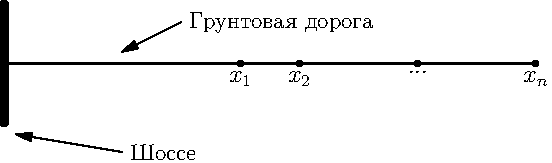
\includegraphics{coop_gadukino.pdf}
\end{figure}





Найдите вектор Шепли.

\vspace{5pt} <<\indef{Нефтепровод}>>

Нефть можно доставить из точки А в точку Б по нефтепроводу. 

%\begin{figure}[htbp]
%\begin{asy}
%
%import unicode;
%texpreamble("\usepackage{mathtext}\usepackage[russian]{babel}");
%defaultpen(font("T2A","cmr","m","n"));
%unitsize (1cm);

%draw("\begin{small}4\end{small}",(0,0)--(1,-1),Arrow);
%draw("\begin{small}1\end{small}",(0,0)--(1,1),S,Arrow);
%draw("\begin{small}3\end{small}",(1,1)--(1,-1),Arrow);
%draw("\begin{small}2\end{small}",(1,1)--(2,0),S,Arrow);
%draw("\begin{small}5\end{small}",(1,-1)--(2,0),Arrow);
%
%dot((0,0));
%label("A",(0,0),W);

%dot((2,0));
%label("B",(2,0),E);

%\end{asy}


%\end{figure}

\begin{figure}[htbp]
	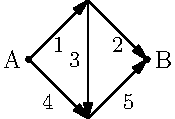
\includegraphics{coop_nefteprovod.pdf}
\end{figure}

Собственники труб и пропускная способность труб в таблице:

\begin{tabular}{|c|c|c|}

\hline 
Номер трубы & Пропускная способность & Владелец \\
\hline
1 & 2 л/час & Андрей \\
2 & 3 л/час & Борис \\
3 & 1 л/час & Володя \\
4 & 2 л/час & Борис \\
5 & 3 л/час & Андрей \\
\hline
\end{tabular}

Потребители нефти готовы платить 1 рубль за скорость передачи 1 литр/час. 

Найдите вектор Шепли.




\section{Ядро и вектор Шепли. Немного теории.}

Мы ответим на несколько вопросов:

Когда ядро не пусто?

Почему вектор Шепли - это хорошо?

Когда вектор Шепли лежит в ядре?

Поехали!

\subsection{Когда ядро не пусто?}

Разрешим каждому игроку трудиться в нескольких коалициях сразу. Каждый игрок будет распределять свое время (усилия) между теми коалициями, членом которых он является. Причем обяжем всех игроков входящих в одну коалицию трудится в ней одинаковое количество времени. К примеру, в коалиции $S_{1}$ все ее члены трудятся 20\% своего времени, в коалиции $S_{2}$ все ее члены трудятся - 30\% своего времени и т.д. 

С помощью $\lambda_{S}$ обозначим долю своего времени (своих сил), которые тратят на коалицию $S$ ее сотрудники. Конечно же, для любой коалиции $S$ величина $\lambda_{S}\in [0;1]$ и для любого игрока $i$: $\sum_{S, i\in S} \lambda_{S}=1$ (все свои усилия игрок куда-то тратит). 

Для простоты введем:
\begin{mydef}
Набор весов $\lambda_{S}$ называется сбалансированным \index{Сбалансированный набор весов}, если $\forall$ $S$ $\lambda_{S}\in[0;1]$ и $\forall i$ $\sum_{S, i\in S} \lambda_{S}=1$.
\end{mydef}

Критерий непустоты ядра довольно прост:

Большая коалиция должна зарабатывать достаточно много, чтобы суметь пообещать каждой коалиции столько, чтобы у той не было желания отсоединиться. А именно:

Ядро не пусто, если и только если при любом распределении усилий игроков между коалициями их заработок не превосходит заработка большой коалиции.

\begin{myth} $[$Бондарева$]$.\index{Теорема Бондаревой} \index{Критерий непустоты ядра}
Ядро игры в характеристической форме непусто, если и только если для любого сбалансированного набора $\lambda_{S}$:
\begin{equation}
\sum_{S} \lambda_{S}v(S)\leq v(N)
\end{equation}
\end{myth}

\begin{proof}
Если ядро непусто, то существует вектор $x$, такой что: $\sum_{i\in S} x_{i}\geq v(S)$ для любой коалиции $S$, а $  \sum_{i\in N} x_{i}= v(N)$.

Следовательно,
\begin{equation}
\sum_{S} \lambda_{S}v(S) \leq \sum_{S} \lambda_{S} \sum_{i\in S} x_{i} =
\sum_{i}x_{i}\sum_{S, i\in S}\lambda_{S}=\sum_{i}x_{i}\cdot 1=v(N)
%\leq \sum_{S} \lambda_{S} \sum_{i\in N} x_{i} = \sum_{i\in N} x_{i} \sum_{S} \lambda_{S} = \sum_{i\in N} x_{i} \cdot 1 = v(N)
\end{equation}

Доказательство в обратную сторону перенесено в приложение, на стр. \pageref{bond.proof}.
\end{proof}


\subsection{Почему вектор Шепли - это хорошо?}

Когда мы говорили о ядре, мы ввели два хороших свойства (эффективность и отсутствие сепаратистских тенденций), его определяющих. А из этих хороших свойств немедленно следует способ нахождения (решение системы неравенств).

Когда же мы говорили о векторе Шепли, мы ввели способ его подсчета (как матожидание). Потом мы доказали, что он также эффективен. А какими еще хорошими свойствами он обладает?

Давайте поговорим о справедливости! Справедливость для нас будет предcтавлена двумя требованиями: одинаковые игроки должны получать одинаковый выигрыш и бесполезные игроки должны получать ноль.

\begin{mydef}
Назовем игрока <<болваном>> \index{Болван} (dummy player\footnote{В Osborne \cite{osborne:cgt} dummy player определен как игрок, который в каждую коалицию приносит ровно свою стоимость $v(i)$ и ни капли больше. Этому игроку логично выдать $v(i)$ и исключить его из дальнейшего участия в дележе. На меньшее такой игрок не согласен сам, а больше ни одна коалиция не захочет ему платить.}), если он не добавляет ценность ни одной коалции. Игрок $i$ болван, если $\forall S$: $v(S\cup i)=v(S)$. В частности, $v(i)=0$.
\end{mydef}

В соответствии с библейским принципом <<Кто не работает, тот да не ест!>> болваны должны получать ноль.

\begin{mydef} \label{no_bolvans} Платеж удовлетворяет условию <<Болваны получают ноль \index{Болваны получают ноль}>>, если (хм, неожиданно) болваны получают ноль.
\end{mydef}

Например, если в игру <<Носки>> добавить Васю без носков, то было бы справедливо, чтобы ему ничего не доставалось при дележе выигрыша. При подсчете вектора Шепли для игрока болвана $i$ оказывается, что $Add(i,\pi)=0$ для любого порядка $\pi$ и, следовательно, $E(Add(i))=0$.

\begin{mydef} \label{symmetry} Платеж удовлетворяет требованию \indef{симметричности}, \index{требование симметричности} если одинаковые игроки получают одинаковый выигрыш.
\end{mydef}
Если два игрока вносят одинаковый вклад во все коалиции, то хочется, чтобы они получали одинаково. Например, в игре <<Ботинки>> у Лени и у Левы по одному левому ботинку. В векторе Шепли они получают одинаковый выигрыш. Для одинаковых игроков $i$ и $j$ величины их вкладов во все коалиции равны, поэтому случайные величины $Add(i)$ и $Add(j)$ имеют одинаковое распределение. Поэтому и их математические ожидания равны.  

Еще одно требование: линейность. Условия эффективности, симметричности и условие <<болваны получают ноль>> можно сформулировать в рамках одной игры. Условие линейности связывает между собой платежи в разных играх. А именно:
\begin{mydef} \label{linearity}
Правило $f$, которое сопоставляет каждой игре\footnote{Напомним, что для полного описания игры достаточно указать ее характеристическую функцию $v$} $v$ некий дележ $f(v)$, называется \indef{линейным}, если выполнены два условия:

1. $f(c\cdot v)=c\cdot f(v)$

2. $f(v_{1}+v_{2})=f(v_{1})+f(v_{2})$
\end{mydef}

Что это означает? 

Первое требование довольно логично. Пусть есть две игры. Одна задана характеристической функцией $v$. А во второй - выигрыши любой коалиции в $c$ раз больше, чем в первой, т.е. выигрыши задаются функцией $c\cdot v$. Если мы придумали какой-то <<справедливый>> дележ для первой игры, $f(v)$, то <<справедливый>> дележ для второй игры должен быть $c\cdot f(v)$.

Второе требование чуть более трудное. Пусть у нас снова есть две игры, $v_{1}$ и $v_{2}$. Мы придумали правило $f$, которое устанавливает <<справедливый дележ>> для каждой игры, $f(v_{1})$ и $f(v_{2})$. А теперь представим, что наши игроки взаимодействуют между собой два раза. Утром - они играют в игру $v_{1}$, а вечером в игру $v_{2}$. Получилась новая комбинировання игра $v$, которую мы обозначаем как сумму игр, $v=v_{1}+v_{2}$. Естественно, коалиция $S$ работая отдельно от всех утром и вечером заработает $v_{S}=v_{1}(S)+v_{2}(S)$. Согласно второму требованию <<справедливый>> дележ в комбинированной игре, $f(v)$, должен равняться сумме <<справедливых>> дележей в утренней и вечерней играх.

\begin{myth}
Единственным дележом удовлетворяющим требованиям \hyperref[Pareto]{эффективности}, \hyperref[linearity]{линейности}, <<\hyperref[no_bolvans]{болваны получают ноль}>> и \hyperref[symmetry]{симметричности} является вектор Шепли.
\end{myth}

\begin{proof}
Мы уже фактически доказали, что вектор Шепли удовлетворяет требованиям эффективности, симметричности и требованию <<болваны получают ноль>>. 

Линейность. Одновременно рассмотрим три кооперативных игры: $v_{1}$, $v_{2}$ и комбинированную игру $v=v_{1}+v_{2}$. Есть некий порядок $ \pi $ формирования большой коалиции. Пусть до входа игрока $i$ уже сформирована коалиция $S$. Добавка $Add_{v}(i,pi)$ в комбинированной игре является суммой добавок в утренней и вечерней играх:
\begin{equation}
Add_{v}(i,pi)=Add_{v_{1}}(i,pi)+Add_{v_{2}}(i,pi)
\end{equation}

Т.к. это верно для любого порядка $ \pi $ формирования большой коалиции, получается, что вклад $ i $-го игрока в комбинированной игре (как случайная величина) распадается в аналогичную сумму: $Add_{v}(i)=Add_{v_{1}}(i)+Add_{v_{2}}(i)$. Берем математическое ожидание: $E(Add_{v}(i))=E(Add_{v_{1}}(i))+E(Add_{v_{2}}(i))$. И получаем линейность вектора Шепли: $\phi_{i}(v)=\phi_{i}(v_{1})+\phi_{i}(v_{2})$.

То, что вектор Шепли удовлетворяет первому свойству: $\phi_{i}(cv)=c\phi_{i}(v)$ - аналогично следует из того, что константу можно выносить за знак математического ожидания.

Пусть теперь какое-нибудь правило дележа удовлетворяет четырем требованиям. Докажем, что это может быть только вектор Шепли.
Для начала докажем это для простых игр.

\begin{mydef}
Игра в характеристической форме называется \indef{простой}\index{Простая игра}, если существует особая коалиция $S$, такая что без ее участия в полном составе нельзя получить ничего, а с ее участием в полном составе можно получить единицу:

\begin{equation}
v(K):=
\begin{cases} 
1, S\subset K \\  
0, S\not \subset K \\
\end{cases}
\end{equation}

\end{mydef}

Иногда простые игры называют олигархическими, а игроков, входящих в особую коалицию $S$ - олигархами\index{Олигархическая игра}.

Поскольку в простой игре все игроки не входящие в $S$ - болваны\footnote{Да, каждый игрок либо олигарх, либо болван.}, то они получают 0 (условие <<болваны получают ноль>>). А игроки входящие в $S$ неразличимы между собой, и поэтому обязаны делить общий заработок $v(N)=1$ поровну (условие эффективности плюс условие симметричности), т.е. получать $\frac{1}{|S|}$.
Значит, для простых игр условия <<болваны получают ноль>>, симметричность и эффективность однозначно определяют дележ. А вектор Шепли им всегда удовлетворяет. Значит в простых играх вектор Шепли - единственное условие удовлетворяющее указанным требованиям.

Рассмотрим произвольную игру в характеристической форме. Она полностью определяется функцией $v$. Функцию $v$ можно записать в виде $v=\sum_{S}\mu(S)v_{S}$, где $v_{S}$ это игра с олигархической коалицией $S$, а $\mu_{S}$ - некоторые коэффициенты. Это не что иное, как разложение вектора с помощью базиса. Оно единственно, но нам даже этот факт не нужен. Для наглядности лишь приведем пример:

\begin{myex}
Разложение игры <<Носки>> на простые игры. $v=60v_{\mbox{Андрей}}+120v_{\mbox{Борис}}+60v_{\mbox{Андрей, Борис}}$.
\end{myex}


Для простых игр существует единственный дележ удовлетворяющий трем условиям (эффективность, симметричность, <<болваны получают ноль>>). Характеристическая функция любой игры получается как линейная комбинация характеристических функций простых игр, значит если от дележа дополнительно потребовать линейность, то дележ получается единственным в любой игре.
\end{proof}

\subsection{Когда вектор Шепли лежит в ядре?}

Есть такой красивое словосочетание <<эффект снежного кома>>. Каков его смысл? Если катить маленький снежок, то он медленно растет, а если катить большой ком снега, то он быстро растет. Эта идея иногда верна и в кооперативных играх. К примеру, Вовочка подбивает Петю бойкотировать контрольную, которую устравивает Марь Иванна. Если бойкотировать контрольную пока согласен только сам Вовочка, то Петя мало что добавит к выигрышу Вовочки. А если бойкотировать уже согласны все в классе кроме Пети, то присоединение Пети к бойкотирующим резко увеличивает их выигрыш.

Возникает следующее определение.
\begin{mydef}
Игра в характеристической форме проявляет <<эффект снежного кома\index{Эффект снежного кома}>> (snowball effect), если для любого игрока $i$ и для любых коалиций $K\subset L$ не содержащих игрока $i$ выполнено условие:
\begin{equation}
v(K\cup i)-v(K)\leq v(L\cup i)-v(L)
\end{equation}
\end{mydef}

Левая часть неравенства - это выигрыш маленькой коалиции $K$ от присоединения Пети, а правая часть - выигрыш крупной коалиции $L$ от присоединения Пети.

Это определение эквивалентно более общепринятому, но менее наглядному определению супермодулярности:
\begin{mydef}
Игра в характеристической форме называется супермодулярной \index{Супермодулярность}\index{Супермодулярная игра} (supermodular или convex\footnote{Слово convex оказывается слишком перегруженным (есть convex set, convex function и пр.), поэтому чтобы избежать путаницы лучше использовать supermodular.}), если для любых коалиций $S$ и $T$:
\begin{equation}
v(S\cup T)+v(S\cap T)\geq v(S)+v(T)
\end{equation}
\end{mydef}

Докажем эквивалентность определений:
\begin{proof}
Пусть игра $v$ - супермодулярна. Пусть $K\subset L$, $i\notin L$. Рассмотрим коалиции $S=(K,i)$ и $T=L$. Применяем супермодулярность:
\begin{equation}
v((K,i)\cup L)+v((K,i)\cap L)\geq v(K,i)+v(L)
\end{equation}
Игрок $i$ не лежит ни в $K$, ни в $L$, поэтому:
\begin{equation}
v(L,i)+v(K)\geq v(K,i)+v(L)
\end{equation}
Что дает определение игры с эффектом снежного кома.

Пусть игра $v$ обладает эффектом снежного кома. Пусть $S$ и $T$ - две произвольные коалиции. 

Шаг 1. Рассмотрим коалиции $K=S\cap T$ и $L=T$. По определению $K\subset L$. Рассмотрим произвольного игрока, $i\in S\backslash T$.
В силу эффекта снежного кома:
\begin{equation}
v(K\cup i)-v(K)\leq v(L\cup i)-v(L)
\end{equation}

Шаг 2. Добавим в коалиции $K$ и $L$ игрока $i$, при этом конечно, $(K,i)\subset (L,i)$. Рассмотрим нового произвольного игрока, $j\in S\backslash T$, $j\neq i$. Применяем эффект снежного кома к $(K,i)\subset (L,i)$:
\begin{equation}
v((K,i)\cup j)-v(K,i)\leq v((L,i)\cup j)-v(L,i)
\end{equation}

Заметьте, что если сложить эти два неравенства, то получится:
\begin{equation}
v(K,i,j)-v(K)\leq v(L,i,j)-v(L)
\end{equation}
Это легко интерпретируется: если два игрока $i$ и $j$ вступают в более крупную коалицию $L\supset K$, то они приносят больший доход.

Продолжая добавлять по одному игроков из $S\backslash T$ и складывая неравенства мы получим, что:
\begin{equation}
v(K\cup (S\backslash T))-v(K)\leq v(L\cup (S\backslash T))-v(L)
\end{equation}
Вспомнив, что $K=S\cap T$, а $L=T$, получаем:
\begin{equation}
v(S)-v(S\cap T)\leq v(T\cup S)-v(T)
\end{equation}
что является определением супермодулярности.
\end{proof}

Игры с <<эффектом снежного кома>> хороши тем, что:

\begin{myth}
Ядро супермодулярной игры непусто
\end{myth}
\begin{proof}

Зафиксируем произвольный порядок формирования большой коалиции $\pi$. Оказывается, что вектор $(Add(1,\pi),Add(2,\pi),....,Add(n,\pi))$ лежит в ядре. Действительно:

Для того, чтобы не перегружать доказательство индексами поступим так. Во-первых, поскольку нумерация игроков произвольна, будем считать, что игроки входят в порядке: 1,2,3..., $n$. Если они входят в другом порядке, то перенумеруем их. Во-вторых, введем обозначение $K_{i}$ - это первые $i$ игроков, $K_{i}=\{1,2,3,...,i\}$. До игрока $i$, естественно успели войти игроки из $K_{i-1}$.

Шаг 1. Рассмотрим произвольную коалицию из одного игрока $i$.

В силу супермодулярности: 
\begin{equation}
v(K_{i-1}\cap i)+v(K_{i-1}\cup i)\geq v(K_{i-1})+v(i) 
\end{equation}

Что равносильно: 

\begin{equation}
v(i)\leq v(K_{i-1}\cup i)-v(K_{i-1})
\end{equation}

Значит, $v(i)\leq Add(i,\pi)$.
Итак, ни один игрок не выиграет, если откажется от предлагаемого дележа и возьмет $v(i)$.

Индукция. Допустим мы доказали, что ни одной коалиции из $k-1$ игрока не выгодно отсоединятся. Рассмотрим произвольную коалицию $K$ из $k$ игроков. В этой коалиции есть игрок с наибольшим номером $m$. Значит $K\subset K_{m}$, но $K\not \subset K_{m-1}$. 

В силу супермодулярности:
\begin{equation}
v(K_{m-1}\cap K)+v(K_{m-1}\cup K)\geq v(K_{m-1})+v(K) 
\end{equation}

Заметив, что $K_{m-1}\cup K=K_{m}$ получаем:

\begin{equation}
v(K_{m-1}\cap K)+v(K_{m})-v(K_{m-1})\geq v(K) 
\end{equation}

Разница $v(K_{m})-v(K_{m-1})$ - это то, что вектор Шепли отдает $m$-му игроку, т.е. $v(K_{m})-v(K_{m-1})=Add(m,\pi)$.

В коалиции $K_{m-1}\cap K$ меньше участников, чем в $K$, значит по предположению индукции ей не выгодно отсоединяться, т.е.
\begin{equation}
\sum_{i\in K_{m-1}\cap K}Add(i,\pi)\geq v(K_{m-1}\cap K)
\end{equation}

Получаем, что:
\begin{equation}
\sum_{i\in K_{m-1}\cap K}Add(i,\pi) + Add(m,\pi)\geq v(K)
\end{equation}

Но в левой части стоит ровно та сумма денег, которая предлагается коалиции $K$, а значит и ей не выгодно отсоединятся.
\end{proof}

Поскольку векторы $(Add(1,\pi),Add(2,\pi),....,Add(N,\pi))$ - это то, что усредняет вектор Шепли мы немедленно получаем:


\begin{myth}
Если игра - супермодулярная, то вектор Шепли лежит в ядре
\end{myth}
\begin{proof}
Ядро задается системой линейных неравенств, значит оно является выпуклым множеством. 

Поскольку для любого фиксированного порядка формирования большой коалиции $\pi$ вектор 
\begin{equation}
(Add(1,\pi),Add(2,\pi),....,Add(N,\pi))
\end{equation}
лежит в ядре, то и весь многогранник, что находится <<между>> этими векторами лежит в ядре. Значит и вектор Шепли, как среднее арифметическое этих векторов-вершин многогранника, также лежит в ядре.
\end{proof}

Более того, в супермодулярных играх ничего кроме этого многогранника в ядро и не входит.

\begin{myth}
Ядро супермодулярной игры - это многогранник \index{Многогранник} с вершинами в $(Add(1,\pi),Add(2,\pi),....,Add(n,\pi))$, где $\pi$ - это всемозвожные порядки формирования большой коалиции.
\end{myth}

Оставим это утверждение без доказательства, но проиллюстрируем. 

Возьмем для примера игру, где Алеша Попович, Добрыня Никитич и Илья Муромец ловят драконов. В одиночку - никто не может поймать, вдвоем они ловят $\alpha$ драконов в час, втроем - одного дракона в час. Если мы формируем коалицию в случайном порядке, то первый входящий получает ноль, второй - $\alpha$, а вклад третьего - $(1-\alpha)$. Соответственно наш многогранник (в данном случае все грани оказались в одной плоскости, так вышло) имеет 6 вершин. Шесть вершин - это векторы из чисел 0, $\alpha$ и $(1-\alpha)$ во всех возможных порядках.


\begin{figure}[htbp]
   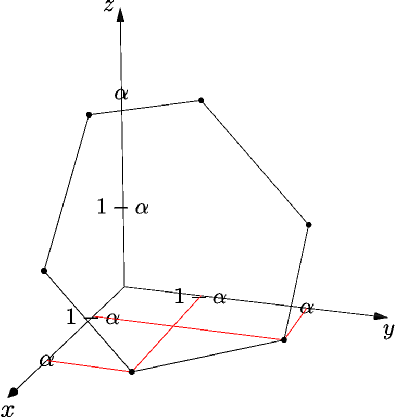
\includegraphics{coop_3player.pdf}
\end{figure}




\subsection{Окончание доказательства т. Бондаревой, критерия непустоты ядра}

Напомним формулировку:
\begin{myth} $[$Бондарева$]$.
Ядро игры в характеристической форме непусто, если и только если для любого сбалансированного набора $\lambda_{S}$:
\begin{equation}
\label{balanced_game2}
\sum_{S} \lambda_{S}v(S)\leq v(N)
\end{equation}
\end{myth}

\begin{proof} \label{bond.proof}

Обратно\footnote{Приведенное доказательство взято из Osborne, Rubinstein, \cite{osborne:cgt}. У Данилова в \cite{danilov:lte} через т. Какутани. Может есть еще более геометрическое доказательство?}. Пусть неравенство \ref{balanced_game2} выполнено.

Для доказательства в обратную сторону нам понадобится технических факт:
\begin{myth}
Два выпуклых множества в $R^{n}$ можно разделить гиперплоскостью. Более алгебраическая формулировка: если есть два выпуклых непересекающихся множества, $A$ и $B$, то существует вектор $\vec{\alpha}$ и число $c$, такие, что для любых $a\in A$ и $b\in B$ верно неравенство: $\vec{\alpha}\cdot b \geq c \geq \vec{\alpha}\cdot a$.
\end{myth}
Этот факт мы примем без доказательства как хорошо согласующийся с геометрическими представлениями.

[Картинка <<и ежу понятно>>]
\begin{figure}[htbp]
	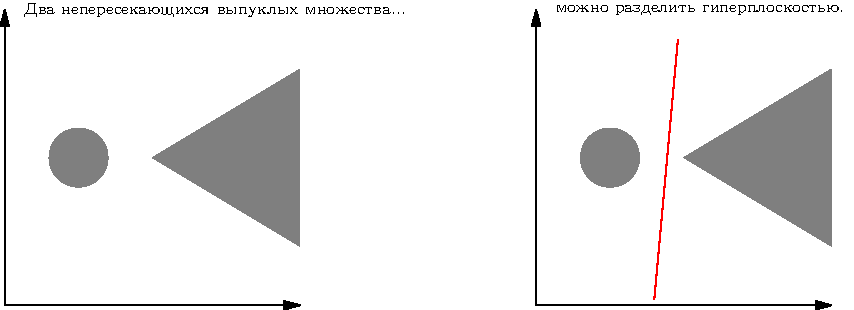
\includegraphics{coop_separating.pdf}
\end{figure}


Введем обозначение $1_{S}$ - это вектор из $n$ чисел, каждое из которых равно нулю или единице, в зависимости от того, входит ли соответствующий участник в коалицию $S$. В частности, $1_{N}$ - это вектор из $n$ единичек, а $1_{\emptyset}$ - это вектор из $n$ нулей. Например, если $N=\{A,B,C,D\}$ и коалиция $S=\{A,D\}$, то $1_{S}=(1,0,0,1)$. Убедитесь, что на этом языке условие сбалансированности набора весов записывается как
\begin{equation}
\sum_{S} \lambda_{S}1_{S}=1_{N}
\end{equation}

Вектор $1_{S}$ лежит в $n$-мерном пространстве.

Допишем к вектору $1_{S}$ стоимость соответствующей коалиции, получим вектор $(1_{S},v(S))$, лежащий в $(N+1)$-мерном пространстве.

Рассмотрим два множества (в $R^{n+1}$):

$A=\{(1_{N},v(N)+\varepsilon)| \varepsilon>0\}$. Это множество выпуклое, т.к. это полупрямая с выколотым началом.

$B=\{\sum_{S} \lambda_{S} (1_{S},v(S)) | \forall  \lambda_{S}\geq 0 \}$. Это множество также выпуклое, т.к. это конус (пирамида). Вершина этого конуса - начало координат. Образующие - векторы вида $(1_{S},v(S))$.


Эти множества не имеют общих точек, в силу неравенства \ref{balanced_game2}. Заметим, что если бы в множестве $A$ была бы разрешена точка c $\varepsilon=0$, т.е. точка $(1_{N},v(N))$, то она и была бы общей.

Для наглядности приведем график\footnote{На самом деле там есть 3d модель, но pdftex из комплекта texlive похоже не может ее присоединить, поэтому пока есть только ее проекция. Если кто знает, как это исправить - напишите.} для двух игроков. Вертикальная ось будет отвечать за $v(S)$. А две остальные оси - за первого и второго игрока. 

\begin{figure}[htbp]
	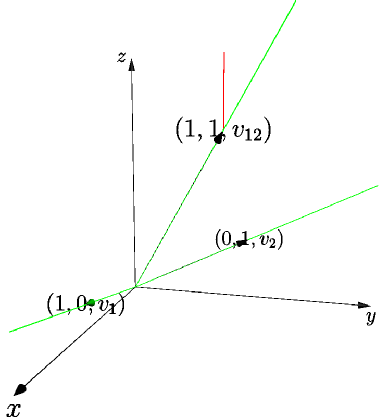
\includegraphics{coop_bondar.pdf}
\end{figure}

Конус с образующими $(1,0,v_{1})$, $(0,1,v_{2})$ и $(1,1,v_{12})$ - это множество $B$, а полупрямая стартующая <<вверх>> из точки $(1_{N},v(N))$ на конусе - это множество $A$. 

 Оба множества выпуклы, значит существует гиперплоскость разделяющая множества $A$ и $B$. Эта гиперплоскость, конечно же проходит через точку $(1_{N},v(N))$. Из рисунка ясно, что можно взять гиперплоскость, содержащую образующую конуса $(1_{N},v(N))$. Т.е. разделяющая гиперплоскость проходит через начало координат. Здесь мы неявно воспользовались супераддитивностью, т.к. нам надо, чтобы образующая $(1_{N},v(N))$ лежала <<выше>> остальных образующих.


В общем случае гиперплоскость определяется ненулевым вектором $\vec{\alpha}=(\alpha_{1},\alpha_{2},...,\alpha_{n+1})$ и числом $c$ так что:

\begin{equation}
	\vec{\alpha}\cdot b \geq c \geq \vec{\alpha}\cdot a
\end{equation},
для любых $a\in A$ и $b\in B$.

В нашем случае есть два уточнения. Поскольку множество $A$ открытое, то правое неравенство можно заменить на строгое.
А поскольку гиперплоскость проходит через начало координат, то константа $c$ равна 0.

Значит применительно к нашему случаю существование разделяющей гиперплоскости выглядит так:

\begin{equation}
\label{hyperplane_eq}
	\vec{\alpha}\cdot b \geq 0 > \vec{\alpha}\cdot a
\end{equation},
для любых $a\in A$ и $b\in B$.


Сначала мы заметим, что $\alpha_{n+1}<0$, а затем построим из $(\alpha_{1},\alpha_{2},...,\alpha_{n})$ элемент ядра.

Разделяющая гиперплоскость проходит через начало координат. Верхняя часть вертикальной оси, т.е. множество $\{(0,...,0,v)|v>0\}$ лежит в той же половине пространства, что и множество $A$. Значит $\alpha_{n+1}\cdot v<0$. Значит $\alpha_{n+1}<0$.

%Заметим, что $\alpha_{n+1}$ не может быть положительным: если бы оно было положительным можно было бы взять вектор $a$ с большим $\varepsilon$ и добиться положительности $\vec{\alpha}\cdot a$.

%Уточним, что $\alpha_{n+1}$ не может быть равен нулю. Для этого рассмотрим вектор $v=(1_{N},v(N))$, начало полупрямой $A$. Он лежит в множестве $B$ - достаточно взять $\lambda_{N}=1$, а остальные $\lambda_{S}=0$. Поскольку вектор $v$ попадает на границу $A$ для него неравенство выглядит так: $\vec{\alpha}\cdot v \geq 0 \geq \vec{\alpha}\cdot v$.

%Заметим, что $\vec{\alpha}\cdot v=\sum_{i=1}^{N}\alpha_{i}+\alpha_{n+1}v(N)$.

%При $\alpha_{n+1}$ равном нулю мы получали бы, что $\sum_{i=1}^{n}\alpha_{i}=0$. Но это невозможно, т.к. в этом случае $\vec{\alpha}\cdot a$ равнялось бы нулю.

Поделим неравенство \ref{hyperplane_eq} на $(-\alpha_{n+1})$. При этом знаки неравенства не поменяются, а последняя компонента вектора $\vec{\alpha}$ превратится в минус единицу. Обозначим: $x_{i}=-\alpha_{i}/\alpha_{n+1}$.

Что это нам дает?

Левая часть неравенства говорит: для любого $b$: $(x_{1},x_{2},...,x_{n},-1)\cdot b \geq 0$.

Возьмем $b=(1_{S},v(S))$. Получаем, $\sum_{i\in S}x_{i}\geq v(S)$.

Правая часть неравенства говорит: для любого $a$: $(x_{1},x_{2},...,x_{n},-1)\cdot a <0$.

Возьмем $v=(1_{N},v(N))$. Этот вектор в $A$ не входит, но лежит на границе $A$, поэтому неравенство будет нестрогим: $\sum_{i\in N}x_{i}\leq v(N)$.

Что это значит? Это означает, что есть такой вектор $x$, который большая коалиция может выплатить (может у нее даже что-то останется). При этом ни одна коалиция $S$ не может получить больше, чем достается ей при дележе $x$. Следовательно, ядро не пусто.

\end{proof}


\subsection{Дз 2}

\vspace{5pt} \indef{Задача 1.}

Какие из рассмотренных примеров игр являются супермодулярными?

Ботинки-2, Малое Гадюкино, 3 player unanimity game, Гномы и золото, Нефтепровод, Угадай цену пирога, Помещик и крестьяне


\vspace{5pt} \indef{Задача 2.}

Приведите пример несупераддитивной игры. Желательно не абстрактный, а жизненный. Желательно смешной.


\vspace{5pt} \indef{Задача 3.}

а) Докажите, что из супермодулярности следует супераддитивность.

б) Приведите пример супераддитивной, но не супермодулярной игры. Желательно не абстрактный, а жизненный. Желательно смешной.


\vspace{5pt} \indef{Задача 4.}

Разложите игры Ботинки, Гномы и золото, Ботинки-2 на простые игры.





\section{Задача торга двух игроков.}

% использовать букву f для выигрыша - исправить в лекции 2 для полноты картины.



\subsection{Определение задачи торга.}

Попробуем разобрать простейший случай, когда полезности не передаются.
У нас будет всего \indef{два} игрока. Либо каждый из них работает
в одиночку, либо формируется большая коалиция. Большая, в данном случае,
- это из обоих игроков.

Соответственно, описание задачи торга состоит из двух объектов:

\begin{mydef} Точка разногласия \index{Точка разногласия} (disagreement point) - это вектор
платежей, получаемых игроками, если кооперации не будет. \end{mydef}

\begin{mydef} Множество доступных платежей \index{Множество доступных платежей} - это множество возможных платежей,
которые могут получить игроки если скооперируются. \end{mydef}

\begin{figure}[htbp]
	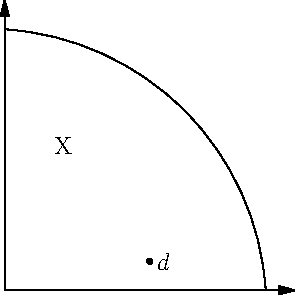
\includegraphics{coop_feasible.pdf}
\end{figure}


С формальной математической точки зрения задача торга задается парой
$(X,d)$, где $X$ - множество доступных платежей, а $d$ - точка разногласия.

Это несколько больше, чем коалиционная игра двух игроков в характеристической
форме. Игра в характеристической форме предполагает, что множество
$X$ имеет вид $X=\{(x_{1},x_{2})|x_{1}+x_{2}\leq v(N)\}$. В задаче
торга множество $X$ в принципе может иметь любую форму. Поэтому можно
считать, что это не деньги, а полезность. В этих лекциях полезность
измеряется в улыбках.

Впрочем, чаще всего предполагают, что множество доступных платежей не совсем
произвольно, а удовлетворяет требованиям:
\begin{itemize}
\item Замкнуто;
\item Выпукло;
\item Ограничено сверху, т.е. существует такая точка $a=(a_{1},a_{2})$
на плоскости, что все множество $X$ лежит юго-западнее точки $a$;
\item Содержит точку $d$.
\end{itemize}
Мы будем считать, что эти требования выполнены.

Что означает решить задачу торга? Для данной конкретной задачи это
означает выбрать наилучшую точку $x^{*}$из $X$. Но нас интересует
не решение конкретной задачи торга, а некое правило которое позволяет
решать любую задачу торга. Наше правило каждой задаче торга $(X,d)$
сопоставляет некий <<наилучший>> дележ $x^{*}$. С математической
точки зрения, правило дележа - это функция $f$. Соответственно, область
определения функции $f$ - это всевозможные задачи торга, т.е. всевозможные
пары $(X,d)$. 

Пусть $x^{*}$ - это предлагаемый игрокам дележ, т.е. $x^{*}=f((X,d))$.

Чего бы мы хотели от хорошего правила дележа $f$?
\begin{itemize}
\item 
\phantomsection \label{irationality}
Индивидуальная рациональность. \index{Индивидуальная рациональность} Каждый игрок должен получать не меньше,
чем в точке разногласия, $x^{*}\geq d$, т.е. $x_{1}^{*}\geq d_{1}$,
$x_{2}^{*}\geq d_{2}$.
\item Эффективность.\index{Эффективность} Дележ $x^{*}$ должен быть Парето-оптимален. Другими
словами, не существует такой точки $x^{'}$, которая была была бы
для обоих игроков не хуже, а кому-то даже лучше. Формально, не существует
такая точка $x^{'}\neq x^{*}$, что $x^{'}\geq x^{*}$.
\item Симметрия. \index{Симметрия} Если игроки одинаковые (т.е. множество $X$ симметрично
относительно прямой $x_{1}=x_{2}$, и в случае разногласия игроки
получают одинаковый выигрыш $d_{1}=d_{2}$), то $x_{1}^{*}=x_{2}^{*}$.
\item 
\phantomsection \label{scale_invariance}
Нечувствительность к смене масштаба. \index{Нечувствительность к смене масштаба} Пусть есть две задачи торга $(X,d)$
и $(X^{'},d^{'})$, которые отличаются масштабом. Скажем в первой
полезность измерялась в улыбках, а во второй - в улыбочках (одна улыбочка
это $10^{-3}$ улыбок). В этом случае хотелось бы, чтобы решения этих
задач также отличались только сменой масштаба. И более формально:
пусть $X'=aX+b$ и $d'=ad+b$, где $a$ и $b$ - произвольные константы.
Мы говорим, что решение $f$ нечувствительно к смене масштаба, если
$f(X')=af(X)+b$.%
\footnote{Это требование называется у В.И. Данилова скалярной ковариантностью.
Страшно, да?%
}
\item 
\phantomsection \label{3_invariance}
Независимость от третьих альтернатив. \index{Независимость от третьих альтернатив} Если при доступных точках $x$,
$y$, $z$ правило выбирало $x$, то при доступных $x$ и $y$ правило
тоже должно выбирать $x$.
\end{itemize}
Существуют ли решение которое всегда удовлетворяет всем этим требованиям?
Правильный ответ в студию!


\subsection{Решение Нэша}

Для начала введем понятие:

\begin{mydef}
Вектор $y$ называется бонусом от кооперации \index{Бонус от кооперации} при дележе $x$, если $y=x-d$.  Это выигрыш игроков от кооперации по сравнению с точкой разногласия,
\end{mydef}

Нэш предложил странное на первый взгляд решение: 

\begin{mydef} \indef{Решение Нэша} \index{Решение Нэша} - это точка $x_{Nash}$, которая
лежит в $X$ и максимизирует произведение бонусов от кооперации. Т.е.
$(x_{1},x_{2})_{Nash}$ максимизирует функцию $f(x_{1},x_{2})=(x_{1}-d_{1})(x_{2}-d_{2})$.
\end{mydef}

\begin{figure}[htbp]
	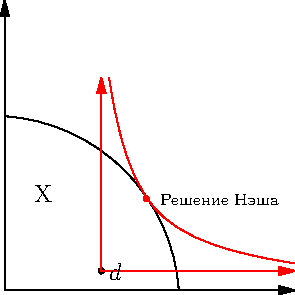
\includegraphics{coop_nash.pdf}
\end{figure}



Давайте попробуем найти решение Нэша в задаче про носки. Напомним
текст:
\begin{myex} Левые и правые носки ничем не отличаются. Пара носков стоит 60 рублей. Один носок ничего не стоит. У Андрея - три носка, у Бориса - пять носков. Здесь $N=\{$Андрей,Борис$\}$, $v($Андрей$)=60$, $v($Борис$)=120$, $v($Андрей, Борис$)=240$.
\end{myex}

В нашем случае, точка несогласия, $d=(60,120)$, а переговорное множество
$X=\{(x_{1},x_{2})|x_{1}+x_{2}\leq240\}$.

Обозначим бонус от кооперации буквой $y_{i}$, т.е. $y_{i}=x_{i}-d_{i}$.
Решение Нэша максимизирует величину $y_{1}\cdot y_{2}$ при ограничении
$y_{1}+y_{2}\leq60$. В силу симметрии $y_{1}=y_{2}=30$.

Значит Нэша предлагает поделить совокупных доход как $(90,150)$.
Что, кстати говоря, совпадает с вектором Шепли и интуитивным дележом
$3:5$.

Оказывается, что:

\begin{myth} Решение Нэша - это единственное решение, удовлетворяющиее
требованиям \hyperref[irationality]{индивидуальной рациональности}, \hyperref[Pareto]{эффективности}, \hyperref[symmetry]{симметричности}, \hyperref[scale_invariance]{нечувствительности к смене масштаба} и \hyperref[3_invariance]{независимости от третьих альтернатив}.
\end{myth}



\begin{proof} 

Для начала рассмотрим задачу торга, где $d=(0;0)$, а переговорное
множество $Y={(x_{1},x_{2})|x_{1}+x_{2}\leq2}$. Игроки симметричны,
значит должны получить одинаковый выигрыш. Единственное симметричное
Парето-оптимальное решение - это $(1,1)$. Решение Нэша именно это и предлагает. 

\begin{figure}[htbp]
	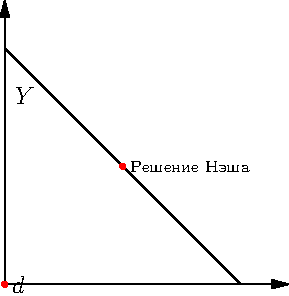
\includegraphics{coop_neproof1.pdf}
\end{figure}



Теперь рассмотрим произвольную задачу торга, $(X,d)$. Идея состоит в том, чтобы так подгадать смену масштаба, чтобы $X'$, отмасштабированное множество доступных альтернатив, оказалось внутри упомянутого множества $Y$ и точка $(1,1)$ была бы у них общей. В силу независимости от третьих альтернатив мы обязаны в отмасштабированном $X'$ выбрать точку $(1,1)$ (она была наилучшей в более крупном множестве $Y$). Значит в исходном множестве $X$ мы обязаны выбирать ту точку, которая после смены масштаба стала точкой $(1,1)$.

\begin{figure}[htbp]
	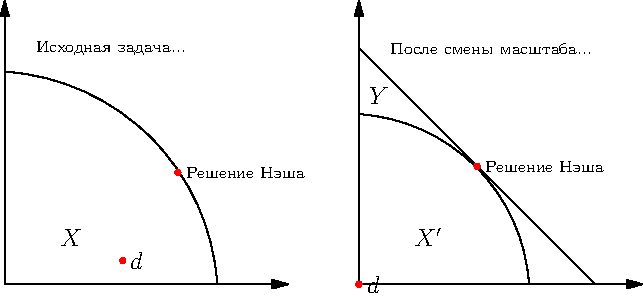
\includegraphics{coop_neproof2.pdf}
\end{figure}


Какая смена масштаба нам нужна? Нужно, чтобы при смене масштаба $d\to (0;0)$ и $x_{NE}\to (1,1)$. Тогда как раз окажется, что правило выбирающее $(1,1)$ в новом $X'$ будет выбирать решение Нэша в исходном $X$. Такая смена масштаба существует. Можно даже предъявить явную формулу (хотя она и не очень нужна, но пусть будет): $x_{i}^{'}=(x_{i}-d_{i})/(x_{NE,i}-d_{i})$. При этом чудесным образом автоматически получается, что новое $X'$ лежит внутри $Y$. 


Почему же окажется, что $X'$ лежит внутри $Y$? На множестве $X$ дележ $x_{NE}$ было равновесием по Нэшу, значит $X$ касалось гиперболы $(x_{1}-d_{1})\cdot (x_{2}-d_{2})=c$. Следовательно, $X$ лежало левее и ниже касательной к этой гиперболе. При смене масштаба касательная аккурат совпадет с прямой $x_{1}^{'}+x_{2}^{'}=2$. В этом можно убедиться выписав ее старое уравнение и сменив масштаб.

\end{proof}


\subsection{Решение Калаи-Смородинского}

Условие независимости от третьих альтернатив может быть рациональным,
но оно зачастую нарушается в реальности. Давайте рассмотрим такой
пример.

Вовочка и Петечка долго спорили о том, кто является самой красивой
девушкой в их классе, Маша или Аня. После долгого спора они пришли
к общему мнению, что самая красивая - Маша. После этого спора Вовочка
и Петечка неожиданно вспомнили про Памеллу Андерсон. А вспомнив про
Памеллу Андерсон, решили, что все-таки, самая красивая - Аня.

На этот пример можно, конечно, возразить, что Памелла Андерсон не
училась в классе Вовочки и Петечки. И это, следовательно, не совсем
независимость от третьих альтернатив. Но идея остается. Чтобы сделать
выбор между несколькими объектами нужно свести многомерные характеристики
объектов к одной единственной лучше-хуже. И вот-это правило сведения
оказывается очень неустойчиво. На него влияет реклама или просто упоминание
третьей альтернативы.

Еще пример. Вы выбирали мобильный телефон и сомневались между А и
Б. И склонились к выбору А. Потом в журнале прочли про то, что есть
такая крутая модель С. Крута она своим дизайном. Вам дизайн С понравился.
И вы сменили свой выбор в пользу Б, потому, что дизайн Б больше похож
на крутой дизайн С. Сама модель С для вас была хуже, чем А и Б, так
как у нее существенно выше цена. Но критерий сведения многомерной
характеристики телефона к одномерному хуже-лучше поменялся просто
из-за самого наличия С.

Решение Калаи-Смородинского заменяет требование независимости от третьих
альтернатив на индивидуальную монотонность. Чтобы проще описать
индивидуальную монотонность определим пару функций:
\begin{itemize}
\item $m_{1}(X,d)$ - это наибольший возможный для первого игрока бонус
от кооперации, при котором бонус второго игрока неотрицателен. И,
аналогично, 
\item $m_{2}(X,d)$ - это наибольший возможный для второго игрока бонус
от кооперации, при котором бонус первого игрока неотрицателей.
\end{itemize}


\phantomsection \label{imonotonicity}
Индивидуальная монотонность (для первого игрока).\index{Индивидуальная монотонность} Допустим у нас есть
две задачи торга, $(X,d)$ и $(X^{'},d^{'})$. Если множество дележей $X^{'}$ больше, чем $X$, но максимальный бонус от кооперации для второго игрока одинаковый, то с точки зрения первого игрока задача $(X^{'},d^{'})$ должна быть лучше задачи $(X,d)$. Формально, если $X\subset X^{'}$ и $m_{2}(X,d)=m_{2}(X^{'},d^{'})$, то $x^{*'}_{1}\geq x^{*}_{1}$.


\begin{mydef}Решение Калаи-Смородинского, $x_{KS}$ - это 
Парето-оптимальное решение, которое делит бонусы от кооперации в пропорции
$m_{1}(X,d):m_{2}(X,d)$.\end{mydef}

\begin{figure}[htbp]
	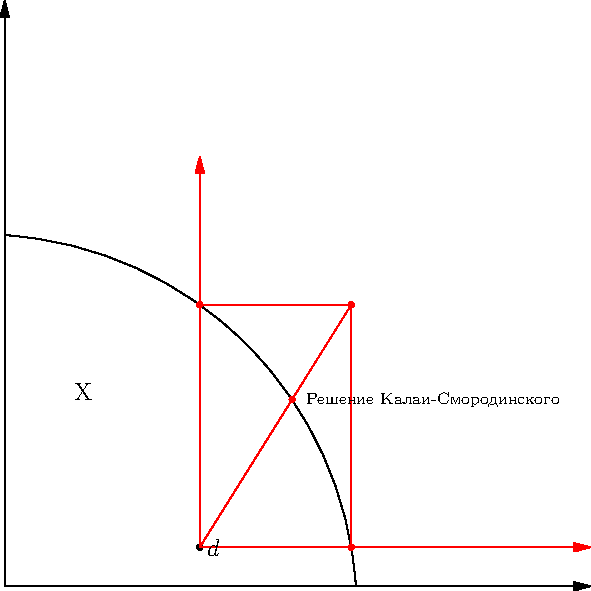
\includegraphics{coop_ks.pdf}
\end{figure}


Как можно было догадаться, верна следующая характеристика решения Калаи-Смородинского:
\begin{myth} Решение Калаи-Смородинского - это единственное решение, удовлетворяющиее
требованиям \hyperref[irationality]{индивидуальной рациональности}, \hyperref[Pareto]{эффективности}, \hyperref[symmetry]{симметричности}, \hyperref[scale_invariance]{нечувствительности к смене масштаба} и \hyperref[imonotonicity]{индивидуальной монотонности}.
\end{myth}

Найдем решение Калаи-Смородинского в задаче про Носки. Точка несогласия,
$(60,120)$. Общий бонус от кооперации - $60$. Поскольку деньги можно
передавать, то максимальный бонус каждого игрока от кооперации также
равен $60$, т.е. $m_{1}=m_{2}=60$. Делим общий бонус от кооперации
в пропорции $60:60$, т.е. поровну. Каждый получает бонус по $30$.
Итоговый дележ $(90,150).$ Что совпадает с решением Нэша, а заодно
и с вектором Шепли.


\subsection{Связь с некооперативной теорией игр.}

Неплохо бы навести какой-то мостик между кооперативной и некооперативной
теориями. Иначе они кажутся совершенно оторванными, хотя решают похожие
задачи.

Представим себе, что торг проходит так:

Период 1. Игрок А предлагает игроку Б любой дележ из $X$. Если Б
согласен, то игра заканчивается. Если игрок Б не согласен, то начинается
период 2.

Период 2. Игрок Б предлагает играку А любой дележ из $X$. Если А
согласен, то игра заканчивается. Если игрок А не согласен, то начинается
период 3.

... и так далее.

Дополнительно добавим в игру ураган. После окончания каждого периода (перед началом следующего) с вероятностью $p\in (0;1)$ начинается ураган. \index{Ураган} В случае урагана игра
принудительно заканчивается и если игроки не успели договориться,
то они получают выигрыш из точки несогласия $d$. Уточним, что дисконтирования
нет.

Зачем нам нужен ураган? Чтобы стимулировать игроков прийти к соглашению
побыстрее. В каком-то смысле он заменяет дисконтирование. Рубль сейчас
лучше чем обещание рубля завтра, т.к. до завтра может начаться ураган
и обещание не будет исполнено.

Найдем равновесие по Нэшу совершенное в подыграх (SPNE) \index{Равновесие по Нэшу совершенное в подыграх} для каждого
$p$. Обозначим вектор платежей, которые получают игроки, как $x_{SPNE}(p)$.

Оказывается, что:

\begin{myth} Решение Нэша в задаче торга является пределом равновесий
по Нэшу совершенных в подыграх, $x_{Nash}=\lim_{p\to 0}x_{SPNE}(p)$.
\end{myth}

\begin{proof}

Как мы уже делали, будем рассматривать бонусы от кооперации. Т.е.,
например, если начался ураган, то игроки получают $(0;0)$. 

Найдем SPNE для произвольного $p$. Если игра дошла до 3-го периода,
то она ничем не отличается от изначальной игры. Поэтому сначала найдем
совсем простое равновесие, в котором предлагаемый каждым игроком дележ
все время один и тот же. Наше равновесие имеет такой вид: При своем
ходе первый игрок всегда будет предлагать один и тот же вектор бонусов
$x^{*}=(x_{1}^{*},x_{2}^{*})$, а второй игрок при своем ходе будет
предлагать вектор бонусов $y^{*}=(y_{1}^{*},y_{2}^{*})$. При этом
$x_{2}^{*}$ - это наименьший бонус, одобряемый вторым игроком, а
$y_{1}^{*}$ - наименьший бонус одобряемый первым игроком. 

Равновесная траектория выглядит так: первый игрок предлагает $x^{*}=(x_{1}^{*},x_{2}^{*})$. Второй игрок соглашается. Игра оканчивается без наступления урагана.

Для поиска SPNE указанного вида применим принцип одноразового отклонения: \index{Принцип одноразового отклонения}

\begin{myth}
Профиль стратегий является равновесием по Нэшу совершенным в подыграх
если и только если ни одному игроку ни в одной подыгре не выгодны
одноразовые отклонения. Под одноразовым отклонением от стратегии $s$
подразумевается любая стратегия $s'$, которая отличается от стратегии
$s$ лишь в один момент времени.\footnote{Для тех, кто плохо помнит, что это значит, приведем пример.
Пусть имеется стратегия $s=\{$в первой партии сделать ход $a$, в последующих
партиях сделать ход, сделанный в первой партии$\}$. Тогда стратегия
$s'=\{$в первой партии сделать ход $b$, в последующих партиях сделать
ход, сделанный в первой партии$\}$ является одноразовым отклонением
от стратегии $s$. Напомним также, что проверять нужно не только равновесную
траекторию, но и любую другую.%
}.

\end{myth}


Проверяем возможность неодобрения высокого платежа. Итак, пусть первый
игрок предложил дележ $x=(x_{1},x_{2}^{*}+\Delta)$, не обязательно
равновесный! Если второй соглашается (согласно своей стратегии), то
он получает бонус $x_{2}^{*}+\Delta$. Если второй игрок делает одноразовое
отклонение (и, стало быть, не соглашается), то: С вероятностью $p$
игроки получают бонус ноль. С вероятностью $(1-p)$ начинается
следующий период, в котором второй игрок (вернувшись к своей стратегии)
предлагает вектор $y=(y_{1}^{*},y_{2}^{*})$ и первый игрок соглашается. 

Чтобы одноразовое отклонение не было выгодно: $x_{2}^{*}+\Delta\geq(1-p)y_{2}^{*}$
для всех $\Delta\geq0$. 

Проверяем возможность одобрения низкого платежа. Итак, пусть первый
игрок предложил дележ $x=(x_{1},x_{2}^{*}-\Delta)$, не обязательно
равновесный! Если второй не соглашается (согласно своей стратегии),
то он получает ожидаемый бонус $(1-p)y_{2}^{*}$. Если второй
игрок делает одноразовое отклонение (и, стало быть, соглашается),
то он получает $x_{2}^{*}-\Delta$.

Чтобы одноразовое отклонение не было выгодно: $(1-p)y_{2}^{*}\geq x_{2}^{*}-\Delta$
для всех $\Delta<0$

Получаем уравнение 

\begin{equation}
\label{eq:spne1}
x_{2}^{*}=(1-p)y_{2}^{*}
\end{equation}

Аналогично для другого игрока, 
\begin{equation}
\label{eq:spne2}
y_{1}^{*}=(1-p)x_{1}^{*}
\end{equation}



Пока что мы получили два уравнения на 4 неизвестных. Еще два получить
совсем просто: бонусы $x^{*}$ и $y^{*}$ в нашем профиле стратегий
должны быть парето-оптимальными, т.к. в противном случае первый игрок
сменит его на $(x_{1}^{*}+\Delta,x_{2}^{*})$, а второй игрок немедленно
одобрит такой дележ.

Честно говоря, надо доказывать, что других существенно отличающихся
равновесий нет, но сейчас мы этого делать не будем.

Итак, при любой вероятности $p$ равновесный (в смысле SPNE)
платеж можно найти из условий:

$x^{*}$ и $y^{*}$ Парето-оптимальны, $x_{2}^{*}=(1-p)y_{2}^{*}$,
$y_{1}^{*}=(1-p)x_{1}^{*}$ 

Это 4 уравнения на 4 неизвестных (Парето-оптимальность означает, что
точки лежат на границе переговорного множества). 

Заметим, что $x_{1}^{*}x_{2}^{*}=y_{1}^{*}y_{2}^{*}$ при любом $p$,
т.е. произведения бонусов, получаемых игроками равны. Графически это
означает, что предложения $x^{*}$ и $y^{*}$ находятся на пересечении
границы переговорного множества и гиперболы $b_{1}b_{2}=const$.
Значение константы $const$ определяется
значением вероятности $p$.


\begin{figure}[htbp]
   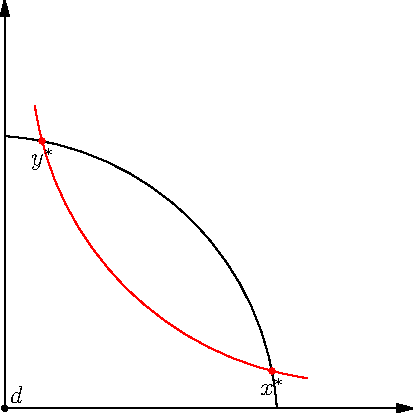
\includegraphics{coop_noncop0.pdf}
\end{figure}


Теперь возьмем произвольную последовательность $p_{n}\downarrow 0$ и посмотрим, что происходит с предложениями $x^{*}(p_{n})$ и $y^{*}(p_{n})$. Из уравнений \ref{eq:spne1} и \ref{eq:spne2} ясно, что точки $x^{*}(p_{n})$ и $y^{*}(p_{n})$ сближаются. Это означает, что гипербола, на которой они лежат сдвигается вправо-вверх. В пределе должны получать единственное решение, и оно совпадает с решением Нэша.

\begin{figure}[htbp]
   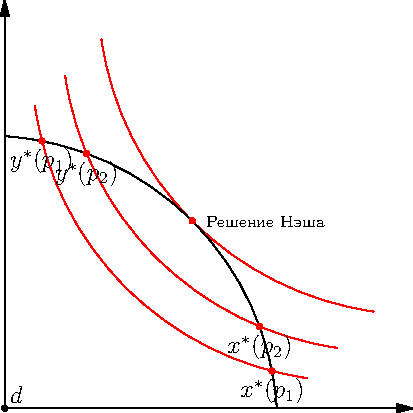
\includegraphics{coop_noncop.pdf}
\end{figure}


\end{proof}



\subsection{Дз 3}

\vspace{5pt} \indef{Задача 1.}
 У первого игрока есть $l$ литров левой полуфилософской
жидкости. У второго игрока есть $m>l$ литров правой полуфилософской
жидкости. При смешивании 1 литра левой и одного литра правой полуфилософской
жидкостей получается 1 кг золота. Полуфилосовская жидкость стоит 1
рубль за литр, золото - 3 рубля за килограмм. Полезность от денег
задана функцией $u(m)=\sqrt{m}$. Как поделить полезность между игроками?
(найдите и решение Нэша и решение Калаи-Смородински).

\vspace{5pt} \indef{Задача 2.}
 Рассмотрим коалиционную игру двух игроков в характеристической
форме.

Верно ли, что решение Нэша всегда совпадает с вектором Шепли? Докажите
или приведите контр-пример.

Верно ли, что решение Калаи-Смородински всегда совпадает с вектором
Шепли? Докажите или приведите контр-пример.

Верно ли, что решение Нэша и Калаи-Смородински всегда совпадают? Докажите
или приведите контр-пример.

\vspace{5pt} \indef{Задача 3.}
 Пусть имеется задача торга $(X,d).$Рассмотрим связанную
с ней некооперативную игру.

Первый игрок предлагает дележ $x^{I}\in X$

Второй игрок предлагает дележ $x^{II}\in X$ и вероятность $p\in[0;1]$.

С вероятностью $p$ игра заканчивается и игроки получают точку несогласия
$d$. С вероятностью $(1-p)$ игра продолжается:

Первый игрок выбирает в качестве финального дележа либо предложенный
им в начале игры дележ $x^{I}$, либо лотерею $px^{II}$. 

Верно ли, что совершенное в подыграх равновесие в этой игре совпадает
с решением Нэша задачи торга? С решением Калаи-Смородински?

\vspace{5pt} \indef{Задача 4.} Докажите, что решение Калаи-Смородинского - единственное
решение, удовлетворяющее условиям эффективности, симметрии, нечувствительности
к смене масштаба, индивидуальной рациональности и индивидуальной монотонности. 

\vspace{5pt} \indef{Задача 5.} Какое решение получится, если известно, что оно удовлетворяет
условиям индивидуальной рациональности, эффективности, симметрии,
индивидуальной монотонности и независимости от третьих альтернатив?

\section{Переговоры.}

В этой главе Винни-Пух узнает несколько решений кооперативных игр, основанных на моделировании переговоров. В этом зачарованном месте мы его и оставим.

На самом деле все подходы к определению равновесия могут быть сформулированы на языке <<возражение-контр-возражение>>. Что такое равновесие по Нэшу в некооперативных играх? Исход, против которого никто в отдельности не возражает. Что такое ядро в кооперативных? Набор платежей, против которого не возражает ни одна коалиция. Проблема заключается в том, что эти концепции оказываются слишком сильными или слишком слабыми. Тогда их можно ослабить или усилить с помощью понятия <<контр-возражения>>.

\subsection{Переговорное множество. Ах если ты так, то я...}

Мы снова возвращаемся к кооперативным играм нескольких игроков в характеристической форме. Несколько следующих концепций решения основаны на моделировании переговоров. Два самых интуитивно понятных требования к дележу - это \hyperref[Pareto]{Парето-оптимальность} и \hyperref[irationality]{индивидуальная рациональность}. Будем рассматривать только те дележи, где эти требования выполнены.

\begin{mydef} \index{Импутация} \indef{Импутация}  (imputation) - любой Парето-оптимальный и индивидуально-рациональный дележ.
\end{mydef}

\begin{mydef}
Импутация $x$ \indef{доступна для коалиции $S$}, если отсоединившись коалиция $S$ может обеспечить своим игрокам выигрыши из импутации $x$, т.е. $\sum_{i\in S}x_{i}\leq v(S)$ или $x(S)\leq v(S)$.
\end{mydef}

Представим себе спор двух игроков, $i$ и $j$ о том, как поделить общественное богатство между всеми игроками (уточним, что всего игроков $n$, а спорят двое). Эти двое будут агитировать разные коалиции за свой дележ.

Предположим, что игрок $j$ предложил импутацию $x$. 

Как ему может возразить игрок $i$? Например, угрозой:

<<Давайте лучше вместо дележа $x$ выберем дележ $y$! А если ты настаиваешь на $x$, то я тогда сколочу против тебя группу $S$, мы отсоединимся и заработаем свою часть дележа $y$ сами, а это больше, чем ты нам предлагаешь в дележе $x$!>>

\begin{mydef}
Пара $(y,S)$ называется \indef{возражением игрока $i$ игроку $j$ на импутацию $x$} если:
\begin{itemize}
\item[-] импутация $y$ доступна для коалиции $S$
\item[-] игрок $i$ входит в $S$, а $j$ не входит в $S$
\item[-] импутация $y$ обеспечивает каждому члену коалиции $S$ более высокий выигрыш чем импутация $x$
\end{itemize}
\end{mydef}

Как игрок $j$ может ответить на это возражение? Например, ответной угрозой: 

<<Если ты пытаешься сколотить группу $S$, то я в ответ сформирую группу $T$, так что им достанется не меньше, чем раньше предлагалось мной или тобой!>>

\begin{mydef}
Пара $(z,T)$ называется \indef{контр-возражением игрока $j$ игроку $i$ на возражение $(y,S)$} если:

\begin{itemize}
\item[-] импутация $z$ доступна для коалиции $T$
\item[-] игрок $j$ входит в $T$, а $i$ не входит в $T$
\item[-] игрокам входящим в $T$ импутация $z$ гарантирует выигрыш не меньший, чем изначальная импутация $x$.
\item[-] игрокам входящим в $T$, и в $S$ импутация $z$ гарантирует выигрыш не меньший, чем обещан возражением $y$.
\end{itemize}
\end{mydef}

Подчеркнем следующий момент. В определение контр-возражения не требуется, чтобы коалиция $T$ пересекалась с коалицией $S$. Если коалиция $T$ из контр-возражения $(z,T)$ пересекается с коалицией $S$, то она действительно мешает формированию коалиции $S$. Но возможна ситуация, когда $T$ не пересекается с $S$ и тогда понятие контр-возражения оказывается довольно слабым. В этом случае игрок $i$ может сказать, <<Ну и ладушки, ты иди со своей $T$, а я пойду со своей $S$, а остальные пусть между собой сами разбираются>>. Это не лишает определение смысла, т.к. в этом случае первый игрок может предложить возражение с коалицией $S\cup T$ и соответствующими платежами.

Используя понятия возражения можно по новому определить ядро:

\begin{mydef}
Ядро \index{Ядро} - это множество импутаций, на которые никто никому не может возразить.
\end{mydef}

Ядро часто бывает пусто, поэтому возникло такое послабление:

\begin{mydef}
Переговорное множество \index{Переговорное множество} - это множество импутаций $x$ таких, что на любое возражение $(y,S)$ игрока $i$ игроку $j$ на $x$, найдется контрвозражение игрока $j$ на возражение $(y,S)$.
\end{mydef}


\begin{myex} Игра <<Носки>>. Индивидуальная рациональность и эффективность дают условия: $x_{1}\geq 60$, $x_{2}\geq 120$, $x_{1}+x_{2}=240$. Далее мы легко замечаем, что ни у кого нет возражений. В этой игре оказалось, что переговорное множество совпало с ядром.
\end{myex}


В общем случае из определения непосредственно вытекает теорема:
\begin{myth}
Ядро всегда лежит в переговорном множестве
\end{myth}

Оказывается, что переговорное множество всегда непусто, что хорошо. Но оказывается внутри него можно выделить K-ядро, которое тоже всегда непусто, а внутри К-ядра еще и единственную точку нуклеолус, которая всегда существует. Более того, в отличие от вектора Шепли, который всегда существует но может не попадать в ядро, нуклеолус всегда существует и попадает в ядро (если, конечно, ядро не пусто). Этим мы сейчас и займемся!

\subsection{К-ядро.}

Сразу скажем, ядро и К-ядро это не одно и то же. В английском это core и kernel. В русском переводе иногда говорят про C-ядро и К-ядро. Мы будем говорить ядро (core) и К-ядро (kernel).

Для краткости определим:
\begin{mydef}
Эксцесс коалиции \index{Эксцесс коалиции} $S$ при импутации $x$ - это разница между суммой, которая коалиция может заработать сама и тем, что ей предлагается в импутации $x$, $e(S,x):=v(S)-x(S)$.
\end{mydef}

Эксцесс можно рассматривать как жертву, приносимую коалицией $S$ при формировании большой коалиции. Если считать, что есть некие издержки формирования коалиции, то вполне логично, что в равновесии эта жертва может быть положительной. Ядро считает, что издержек формирования коалиции нет, и для любой импутации $x$ из ядра эксцесс любой коалиции неположительный.

Заметим, что эксцесс также можно рассматривать как силу коалиции. Если при дележе $x$ у коалиции $S$ большой эксцесс, то у нее больше стимулов уходить, чтобы ее удержать надо менять $x$ в ее пользу.

Чтобы мотивировать К-ядро представим снова представим себе спор двух игроков. Игрок $j$ предложил импутацию $x$. 

Игрок $i$ недоволен и говорит примерно так: 

<<Вот ты, $j$, при дележе получаешь больше чем в одиночку можешь заработать ($x_{j}>v(j)$), а коалиция $S$, где я есть, а тебя - нет, жертвует аж целых $e(S,x)$!!!>>

\begin{mydef}
Коалиция $S$ называется \indef{возражением игрока $i$ игроку $j$} если:
\begin{itemize}
\item[-] игрок $i$ входит в $S$, а $j$ не входит в $S$
\item[-] игрок $j$ получает в импутации $x$ больше, чем может заработать в одиночку, $x_{j}>v(j)$
\end{itemize}
\end{mydef}

На что игрок $j$ возражает,

<<Ха, да коалиция $T$ куда вхожу я, а ты - не входишь, жертвует не меньше!>>

\begin{mydef}
Коалиция $T$ называется \indef{контр-возражением игрока $j$ игроку $i$ на возражение $S$} если:
\begin{itemize}
\item[-] игрок $j$ входит в $S$, а $i$ не входит в $S$
\item[-] эксцесс коалиции $T$ не меньше эксцесса коалиции $S$, $e(T,x)\geq e(S,x)$
\end{itemize}
\end{mydef}


И мы опять потребуем того, чтобы на всякое возражение нашлось контр-возражение:

\begin{mydef}
К-ядро \index{К-ядро} (kernel) - это множество импутаций $x$, таких что на любое возражение $S$ игрока $i$ игроку $j$, игрок $j$ может контр-возразить $T$. 
\end{mydef}


Можно определить К-ядро другим эквивалентным способом. Когда требование индивидуальной рациональности выполнено, игроки делятся на двух типов\footnote{Желающие могут упростить определение в Википедии, ибо два неравенства - это ужас!}: тех, которые получают ровно столько, сколько могут заработать самостоятельно, и тех, которые получают больше. К тем, кто получает ровно столько, сколько может заработать сам, не придерешься. А вот остальные должны как-то мотивировать свой доход. К-ядро требует, чтобы те, кто получает больше чем может заработать сам, были членами коалиций с большим эксцессом. Более формально:

Обозначим с помощью $s_{ij}$ наибольшую возможную жертву, которую приносят коалиции, содержащие игрока $i$ и не содержащие игрока $j$:

\begin{equation}
s_{ij}(x):=\max\{e(S,x)|i\in S,j\notin S\}
\end{equation}

Эту величину можно рассматривать как силу, с которой игрок $i$ может убеждать игрока $j$. 

\begin{mydef}
\indef{К-ядро} \index{К-ядро} (kernel) \index{Kernel} - это множество импутаций $x$, таких, что для любой пары игроков $i$ и $j$ выполнено \indef{хотя бы одно} из двух условий:
\begin{itemize}
\item[-] игрок $j$ получает ровно столько, сколько может заработать, если отсоединится, $x_{j}=v(j)$.
\item[-] игрок $j$ способен убеждать игрока $i$ не меньше, чем игрок $i$ способен убеждать игрока $j$, $s_{ji}(x)\geq s_{ij}(x)$.
\end{itemize}
\end{mydef}

\begin{myex} Игра <<Носки>>. Индивидуальная рациональность и эффективность дают условия: $x_{1}\geq 60$, $x_{2}\geq 120$, $x_{1}+x_{2}=240$. Эксцесс для первого игрока: $(60-x_{1})$, эксцесс второго игрока: $(120-x_{2})$.

Проверяем краевые решения: 

Если $x_{1}=60$, то $x_{2}=180$ и остается проверить, что второй игрок способен убеждать первого сильнее чем первый второго: $120-180\geq 60-60$. Невозможно.

Если $x_{2}=120$, то $x_{1}=120$ и остается проверить, что первый игрок способен убеждать второго, сильнее чем второй первого: $60-120\geq 120-120$. Невозможно.

Внутреннее решение. Силы убеждения должны быть равны. $60-x_{1}=120-x_{2}$. В данном случае К-ядро состоит из единственной точки $(90,150)$.
\end{myex}

Как и было обещано:

\begin{myth}
В кооперативной игре в характеристической форме К-ядро всегда лежит в переговорном множестве.
\end{myth}
\begin{proof}
Рассмотрим произвольную импутацию $x$ из К-ядра. Чтобы доказать, что она лежит в переговорном множестве достаточно предъявить контр-возражение $(z,T)$ на любое возражение $(y,S)$.

Пусть $(y,S)$ возражение игрока $i$ игроку $j$.
\begin{itemize}
\item Если игрок $j$ при дележе $x$ получает ровно столько, сколько может заработать сам, то в качестве контр-возражения годится пара $(z,T)$, где $z=x$, а $T$ состоит только из игрока $j$. В споре это аргумент типа <<Да ты, $i$, глянь, я же себе вообще ничего общественного не взял!>>.
\item Если игрок $j$ при дележе $x$ получает больше, чем может заработать сам, $x_{j}>v(j)$, то в качестве контр-возражения подойдет пара $(z,T)$, где $T$ - коалиция с наибольшим эксцессом среди всех коалиций, содержащих $j$, но не содержащих $i$. Давайте убедимся в этом. Итак, $v(T)-x(T)=s_{ji}(x)$. 

Из того что $x$ лежит в К-ядре следует:
\begin{equation}
v(T)-x(T)=s_{ji}(x) \geq s_{ij}(x)
\end{equation}

Т.к. $s_{ij}$ - максимальный эксцесс:
\begin{equation}
s_{ij}(x) \geq v(S)-x(S)
\end{equation}

Т.к. импутация $y$ доступна для коалиции $S$:
\begin{equation}
v(S)-x(S)\geq y(S)-x(S)
\end{equation}

Неравенство $v(T)\geq x(T)+y(S)-x(S)$ легко довести до готовности напильником:

Во-первых, 
\begin{equation}
y(S)=y(S\cap T)+y(S\backslash T)
\end{equation}

Во-вторых,
\begin{equation}
x(T)-x(S)=(x(S\cap T)+x(T\backslash S))-(x(S\cap T)+x(S\backslash T))=x(T\backslash S)-x(S\backslash T)
\end{equation}

Следовательно, 
\begin{equation}
v(T)\geq y(S\cap T)+y(S\backslash T)+x(T\backslash S)-x(S\backslash T)
\end{equation}. 

По определению возражения, $y(S\backslash T)-x(S\backslash T)\geq 0$. Значит $v(T)\geq y(S\cap T) + x(T\backslash S)$. А это и означает, что у коалиции $T$ хватит денег, чтобы заплатить своим членам не меньше, чем они получают при $x$, а тем членам, кого соблазняли возражением $(y,S)$ заплатить не ниже того, что обещано при дележе $y$, т.е. соответствующий $z$ существует.
\end{itemize}


\end{proof}

Отметим, что переговорное множество, как и обычное ядро легко обобщаются на случай игры с нетрасферабельной полезностью. Связано это с тем, что переговорное множество и ядро не сравнивают полезности разных коалиций, а К-ядро сравнивает. Поэтому эта теорема не обобщается на игры с нетрансферабельной полезностью. 

\subsection{Нуклеолус}

Еще одна пара возражение-контрвозражение. На этот раз представим спор двух коалиций, $S$ и $T$. Коалиция $T$ предложила импутацию $x$.

Коалиция $S$ может возразить:

<<Давайте лучше выберем дележ $y$, т.к. мы получим при этом больше денег, $y(S)>x(S)$!>>
\begin{mydef}
Пара $(S,y)$ называется возражением коалиции $S$ на дележ $x$, если при дележе $y$ коалиция $S$ получает больше, чем при дележе $x$, $y(S)>x(S)$.
\end{mydef}

На что коалиция $T$ может контр-возразить:

<<Разбежались! В своем дележе вы нас аж дважды обидели! Мало того, что мы меньше получаем, $y(T)<x(T)$, так еще и наши стимулы отсоединяться становяться больше, чем были ваши при изначальном дележе, $e(T,y)\geq e(S,x)$.>>
\begin{mydef}
Коалиция $T$ называется контр-возражением на возражение $(S,y)$, если:
\begin{itemize}
\item[-] коалиция $T$ получает при дележе $y$ меньше, чем при дележе $x$, $y(T)<x(T)$
\item[-] эксцесс коалиции $T$ при дележе новом дележе $y$ больше, чем эксцесс коалиции $S$ при дележе $x$, $e(T,y)\geq e(S,x)$
\end{itemize}
\end{mydef}


\begin{mydef}
Нуклеолус \index{Нуклеолус} - это множество импутаций $x$ таких, что на любое возражение $(S,y)$ на $x$ найдется контр-возражение $T$.
\end{mydef}


\begin{myex} Рассмотрим игру <<Носки>>. Пара носков стоит 60 рублей. Один носок ничего не стоит. У Андрея - три носка, у Бориса - пять носков, поэтому $N=\{$Андрей,Борис$\}$, $v($Андрей$)=60$, $v($Борис$)=120$, $v($Андрей, Борис$)=240$. 

Пусть $x$ - импутация. Пусть на эту импутацию есть возражение $y$ от первого игрока, т.е. $y_{1}>x_{1}$. Когда у второго будет контр-возражение? Для контр-возражения нужно, чтобы он получал меньше и чтобы его эксцесс становился больше, чем был у первого. Импутации $y$ и $x$ эффективны, первый получает больше при $y$, значит второй автоматом получает меньше при $y$. Эксцесс второго при $y$ равен $(120-y_{2})=120-(240-y_{1})=y_{1}-120$, эксцесс первого при $x$ равен $60-x_{1}$.

Итого: из неравенства $y_{1}>x_{1}$ должно следовать $y_{1}-120\geq 60-x_{1}$.

Аналогично для возражения второго и контр-возражения первого:

Из неравенства $y_{1}<x_{1}$ должно следовать $60-y_{1}\geq x_{1}-120$.

Значит $x_{1}=180-x_{1}$. Следовательно, нуклеолус - это $(90,150)$. Что говорит в пользу нуклеолуса, т.к. снова соответствует интуитивному дележу 3:5.
\end{myex}

\begin{myth}
Нуклеолус всегда всегда существует и состоит из одной точки.
\end{myth}

\begin{myth}
Нуклеолус всегда лежит в К-ядре
\end{myth}

Из этих двух теорем непосредственно следует, что К-ядро всегда непусто, а следовательно и переговорное множество всегда непусто.

\begin{myth}
Если ядро непусто, то нуклеолус лежит в ядре.
\end{myth}

Мы оставим доказательства этих трех теорем за пределами нашего краткого курса. Но (опять же без доказательств) мы дадим другое описание нуклеолуса, чтобы стало понятнее, что же это за зверь, и почему эти теоремы похожи на правду.

Когда задана импутация $x$ для каждой коалиции можно выписать ее эксцесс. Упорядочим эксцессы по убыванию. Получим, что каждой импутации $x$ однозначно сопоставлен вектор эксцессов $E(x)=(e(S_{1},x),e(S_{2},x),...)$, где $e(S_{k},x)\geq e(S_{k+1},x)$.

Большие значения эксцессов означают нестабильность дележа $x$: чем больше эксцессы, тем больше стимулов у коалиций отказаться от дележа $x$. Поэтому равновесным логично считать дележ с наименьшим вектором эксцессов. Вопрос лишь в том, как сравнить два вектора с разными числами, где иногда больше компонента первого вектора, а иногда - второго.

В начале вектора $E(x)$ идут более крупные, следовательно, более важные эксцессы. Поэтому разумно сравнивать векторы эксцессов по лексикографическому принципу:

\begin{mydef}
Вектор $a$ \indef{лексикографически больше} \index{Лексикографический принцип} вектора $b$ если первая несовпадающая цифра больше в векторе $a$.
\end{mydef}

Пример: вектор (5,5,4,4,1) лексикографически больше вектора (5,4,4,4,4).

Оказывается можно дать такое определение нуклеолуса:
\begin{mydef}
Нуклеолус \index{Нуклеолус} - это дележ с самым маленьким (в лексикографическом смысле) вектором эксцессов.
\end{mydef}


Доказать эквивалентность данных двух определений нуклеолуса непросто. Зато из второго определения легко следует его существование, единственность и способ нахождения. Сейчас мы его и продемонстрируем.

Почему ядро бывает пусто? Потому, что оно требует, чтобы эксцесс любой коалиции не превосходил бы ноль. Естественно, можно ослабить эти неравенства и рассмотреть более широкое $\varepsilon$-ядро:

\begin{mydef}
$\varepsilon$-ядро \index{$\varepsilon$-ядро} - это множество импутаций $x$, таких что эксцесс любой коалиции не превосходит $\varepsilon$, т.е. для любой $S$ верно неравенство $e(S,x)\leq \varepsilon$.
\end{mydef}

Другими словами, $\varepsilon$-ядро - моделирует ситуацию, когда ни одной коалиции не выгодно отсоединяться, при условии, что издержки отсоединения равны $\varepsilon$. По определению, ядро является $0$-ядром. 

Допустим, что ядро пусто. Будем увеличивать $\varepsilon$ до тех пор пока в $\varepsilon$-ядре не появится какой-нибудь дележ. такой момент рано или поздно наступит, поскольку заработок любой коалиции ограничен заработком большой коалиции $v(N)$. Поскольку неравенства нестрогие, будет существовать и наименьшее $\varepsilon$ при котором $\varepsilon$-ядро непусто.

\begin{mydef}
Около-ядро \index{Около-ядро} (near-core, least-core) - наименьшее непустое $\varepsilon$-ядро.
\end{mydef}

Оказывается нуклеолус можно нащупать в около-ядре таким способом:

Начнем с около-ядра. 

Шаг 1. Запомним наименьшее $\varepsilon$ и те коалиции, для которых дальнейшее уменьшение $\varepsilon$ приводит к пустоте $\varepsilon$-ядра. Этим коалициям при дальнейшем увеньшении $\varepsilon$ выгодно отсоединится.
Получим некое пороговое $\varepsilon_{1}$ и некий список коалиций $B_{1}$, для которых это $\varepsilon_{1}$ является наименьшими издержками для невыгодности выхода из большой коалиции. Снижая $\varepsilon$ мы добились, что ни один эксцесс не превосходит $\varepsilon_{1}$ и улучшить этот результат нельзя.

Шаг 2. Для остальных коалиций будем уменьшать $\varepsilon$ в неравенстве $e(S,x)\leq \varepsilon$. Наступит такой момент, что дальнейшей уменьшение $\varepsilon$ снова приводит пустоте множества дележей, т.к. некоторым другим коалициям становится выгоднее отсоединиться.
Получим некое $\varepsilon_{2}$ и некий список коалиций $B_{2}$. Сейчас мы добились того, что все эксцессы (кроме тех, что нельзя сделать ниже $\varepsilon_{1}$) не превосходят $\varepsilon_{2}$.

Шаги 3-... Будем повторять шаг 2 до тех пор, пока дальнейшее уменьшение $\varepsilon$ хотя бы для одной коалиции будет приводит к пустоте множества дележей.

В результате получаем некий единственный дележ. Он будет единственным т.к. в противном случае, можно было бы <<урезать>>  множество снизив $\varepsilon_{k}$ в одном из неравенств. По построению мы получили лексикографически минимальный элемент. Значит это нуклеолус.


Помимо этого дележа получаем убывающую последовательность эксцессов $\varepsilon_{1}$, $\varepsilon_{2}$, ... и непересекающиеся списки коалиций $B_{1}$, $B_{2}$, ... Число коалиций в списке $B_{i}$ обозначим как $b_{i}$. Нуклеолусу будет соответствовать вектор эксцессов:

\begin{equation}
(\underbrace{\varepsilon_{1},\varepsilon_{1} ..., \varepsilon_{1}}_{\mbox{$b_{1}$ раз}}, \underbrace{\varepsilon_{2},\varepsilon_{2} ..., \varepsilon_{2}}_{\mbox{$b_{2}$ раз}}, ...) 
\end{equation}


\begin{myex} Покажем эту процедуру на примере игры <<Носки>>.

Пусть $x$ - импутация, т.е. $x_{1}+x_{2}=240$, $x_{1}\geq 60$, $x_{2}\geq 120$.

Мы должны минимизировать наибольший эксцесс, $\min \varepsilon$ при ограничениях:

$60-x_{1}\leq \varepsilon$ и $120-x_{2}\leq \varepsilon$

Находим, что $\varepsilon_{1}=-30$. При этом оба неравенства превращаются в равенство. Т.е. решение получилось уже после первого шага. Нуклеолус, как и при первом способе, равен $(90,150)$. Вектор эксцессов, $E(x)=(-30,-30)$.
\end{myex}

Если верить в эквивалентность двух определений нуклеолуса, то теорема о том, что нуклеолус лежит в ядре, если оно непусто, оказывается автоматически доказанной, т.к. в этом случае первый шаг начинается с ядра.



\subsection{Решение Неймана-Моргенштерна. С чего все начиналось?}

Осталось лишь рассказать об одной из первых концепций решения кооперативных игр. Речь идет об устойчивом множестве (решении Неймана-Моргенштерна). Для этого нам потребуется еще одно понятие возражения. 

\begin{mydef}
Импутация $y$ называется \indef{возражением коалиции $S$ на импутацию $x$} если: 
\begin{itemize}
\item[-] импутация $y$ обеспечивает каждому члену коалиции $S$ более высокий выигрыш чем импутация $x$
\item[-] импутация $y$ доступна для коалиции $S$, $v(S)\geq y(S)$.
\end{itemize}
Обозначаем $y\succ_{S} x$
\end{mydef}

Используя это понятие, легко например определить уже известное нам ядро:

\begin{mydef}
\index{Ядро} - это множество всех импутаций, на которые ни у одной коалиции нет возражения.
\end{mydef}

Чуть ослабив требования мы получим решение Неймана-Моргенштерна (устойчивое множество)

\begin{mydef}
Множество импутаций $Y$ называется решением Неймана-Моргенштерна или устойчивым множеством \index{Решение Неймана-Моргенштерна} \index{Устойчивое множество} (stable set, NM-solution) если выполнены два условия:

Внутренняя стабильность \index{Внутренняя стабильность}: Если $x$ и $y$ - две импутации из $Y$, то не существует коалиции $S$ для которой $y$ было бы возражением на $x$.

Внешняя стабильность \index{Внешняя стабильность}: Если $x$ - импутация не входящая в $Y$, то найдется коалиция $S$, которая сможет предъявить в качестве возражения на $x$ некоторую импутацию $y$ из $Y$.
\end{mydef}

Сразу заметим, что устойчивых множеств может быть много. Устойчивое множество представляет собой разбиение множества возможных импутаций на две части: импутации внутри $Y$ не являются возражением друг на друга ни с чьей точки зрения, а на импутации вне $Y$ можно найти возражение из $Y$ (с чьей-нибудь точки зрения). Впрочем, импутации извне $Y$ могут быть возражениями на импутации внутри $Y$, это не запрещается.

\begin{myex}
Илья Муромец, Добрыня Никитич и Алеша Попович охотятся на одного единственного Змея Горыныча. В одиночку никто не может его поймать. А любые два богатыря уже могут поймать Змея Горыныча.

$A=\{(0.5,0.5,0),(0.5,0,0.5),(0,0.5,0.5)\}$ - это устойчивое множество. Проверяем внутреннюю стабильность. В одиночку игроки возражать не могут, т.к. не могут завалить Змея Горыныча. А среди данных дележей нет варианта, чтобы при смене $x$ на $y$ становилось лучше сразу двум игрокам. Проверяем внешнюю стабильность. Пусть есть некий дележ $z$ не равный этим трем. Тогда в этом дележе $z$ обязательно найдется два игрока, получающих строго меньше половины. И дележ $z$ будет доминироваться дележом из $A$, где эти двое получают по 0.5.

$B=\{(0.3,x_{2},x_{3}|x_{2}+x_{3}=0.7\}$ - тоже устойчивое множество. Проверяем внутреннюю стабильность. Снова в одиночку никто не может ничего получить, а увеличить сразу два платежа невозможно. Проверяем внешнюю стабильность. Пусть есть некий дележ $z$ не входящий в $B$. Если в дележе $z$ первый игрок получает больше 0.3, то мы его сможем доминировать дележом, где второй и третий игроки получают больше, чем в $z$. Допустим в дележе $z$ первый игрок получает меньше 0.3. Рассмотрим два дележа из $B$: $(0.3,0.7,0)$ и $(0.3,0,0.7)$. Один из них обязательно доминирует $z$, т.к. первому игроку любой дележ из $B$ предпочтительнее, а одновременное выполнение неравенств $z_{2}\geq 0.7$ и $z_{3}\geq 0.7$ невозможно.

Упражнение. Какие еще устойчивые множества есть в этой игре?
\end{myex}

Устойчивые множества не могут быть вложены друг в друга:
\begin{myth}
Если $X$ - устойчивое множество, то не существует устойчивого множества $Y$ целиком лежащего внутри $X$ и не совпадаюющего с $X$.
\end{myth}
\begin{proof}
Допустим, что $Y$ целиком лежит в $X$ и не совпадает с $X$. Значит можно выбрать две точки $x\neq y$, так, что $x\in X\backslash Y$, $y\in Y$. Получаем, что с одной стороны, $y$ должно быть возражением на $x$ (внешняя стабильность $Y$), а с другой стороны, $y$ не может быть возражением на $x$ (внутренняя стабильность $X$). Противоречие.
\end{proof}


\begin{myth}
Любое устойчивое множество содержит внутри себя ядро. Если ядро является устойчивым множеством, то других устойчивых множеств не существует.
\end{myth}
\begin{proof}
Определение ядра более строгое, чем определение устойчивого множества: в первом случае не должно быть ни одного возражения, во втором случае на возражения наложены ограничения. Поэтому ядро входит в любое устойчивое множество.

Как мы только что доказали, устойчивые множества не могут быть вложены друг в друга, а ядро входит в каждое устойчивое множество. Значит если ядро само по себе устойчиво, то других устойчивых множеств быть не может.
\end{proof}

К сожалению, решение Неймана-Моргенштерна иногда бывает пусто. Контрпример в виде игры с 10 игроками есть в статье Лукаса \cite{lucas:gns}.
\nocite{lemaire:cgtia}





\subsection{Дз 4}

Подозрительно похоже на дз 1 ;)

\vspace{5pt} <<\indef{Ботинки-2}>>. Есть $n$ игроков, каждый из которых владеет левым ботинком, и есть еще $m$ игроков, каждый из которых владеет правым ботинком, $n>m$. Каждый левый подходит к каждому правому. Одна полная пара ботинок стоит 1 рубль.  

Опишите переговорное множество, К-ядро и нуклеолус

\vspace{5pt} <<\indef{Гномы и золото}>>. Группа из $n$ гномов нашла много золотых слитков в пещере. Начинается обвал, поэтому нужно срочно убегать из пещеры. После обвала пещера окажется недоступной. Слитки золота тяжелы: в одиночку ни один гном не может нести слиток, но два гнома могут свободно нести один слиток. Снаружи пещеры слитки золота можно продать по цене 1 рубль за штуку. 

Опишите переговорное множество, К-ядро и нуклеолус

\vspace{5pt} <<\indef{Угадай цену пирога}>>
От пирога остался один кусочек. На него претендуют три брата. Папа предлагает им по очереди попробовать угадать цену пирога: сначала гадает старший, затем - средний и в конце - младший. Братья знают, что цены пирогов распределены равномерно на $[0;1]$. 
\begin{itemize}
\item Опишите переговорное множество, К-ядро и нуклеолус
\item Найдите все устойчивые множества
\end{itemize}


\vspace{5pt} <<\indef{Помещик и крестьяне}>>
Есть один помещик и $n$ крестьян. Помещик владеет полем. Без поля крестьяне не могут ничего заработать. Если помещик предоставил поле и на нем работают $k$ крестьян, то они получают выгоду $f(k)$, где $f$ - функция с $f'>0$. 

Найдите нуклеолус


\vspace{5pt} <<\indef{3 player unanimity game}>>
Илья Муромец, Алеша Попович и Добрыня Никитич охотятся на Змеев-Горынычей. В одиночку никто из них не может одолеть ни одного Змея-Горыныча. Втроем - могут одолеть одного Змея-Горыныча за час, вдвоем - $\alpha\in (0;1)$ Змеев-Горынычей за час.

\begin{itemize}
\item Опишите переговорное множество, К-ядро и нуклеолус
\item Найдите все устойчивые множества
\end{itemize}

\vspace{5pt} <<\indef{Малое Гадюкино}>>
От шоссе до деревни Малое Гадюкино идет грунтовая дорога. Осенью дорога приходит в ужасное состояние, поэтому Малые Гадюкинцы на общем собрании решили заасфальтировать ее. При распределении затрат необходимо учесть тот факт, что деревня растянута вдоль дороги, и фактически Гадюкинцы живут на разных расстояниях от шоссе. Всего в Малом Гадюкино обитает  $n$  семей, на расстояниях от шоссе равных  $x_{1}$,  $x_{2}$,...  $x_{n}$ метров. За 1 рубль можно заасфальтировать 1 метр.


\begin{figure}[htbp]
    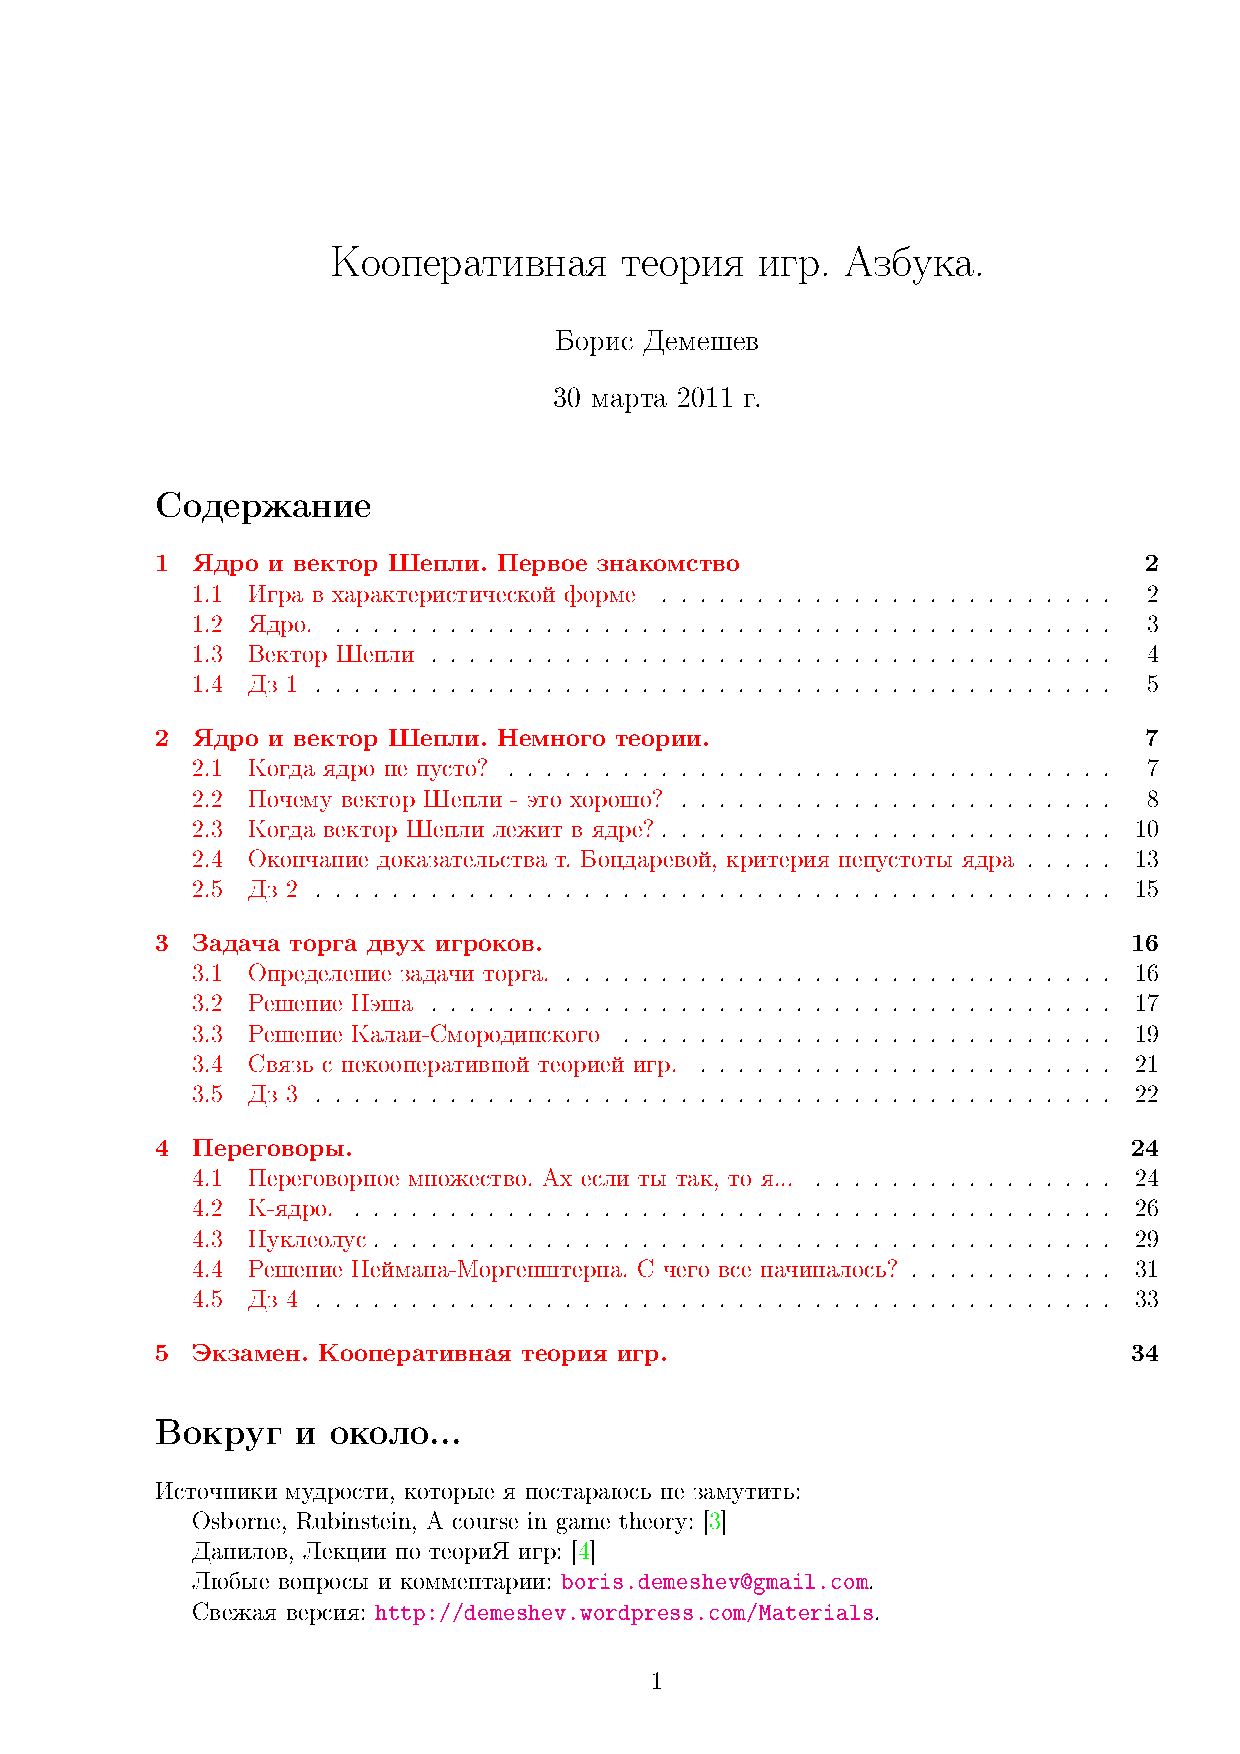
\includegraphics{coop_gt.1}
\end{figure}


Найдите нуклеолус


\vspace{5pt} <<\indef{Нефтепровод}>>

Нефть можно доставить из точки А в точку Б по нефтепроводу. 

\begin{figure}[htbp]
    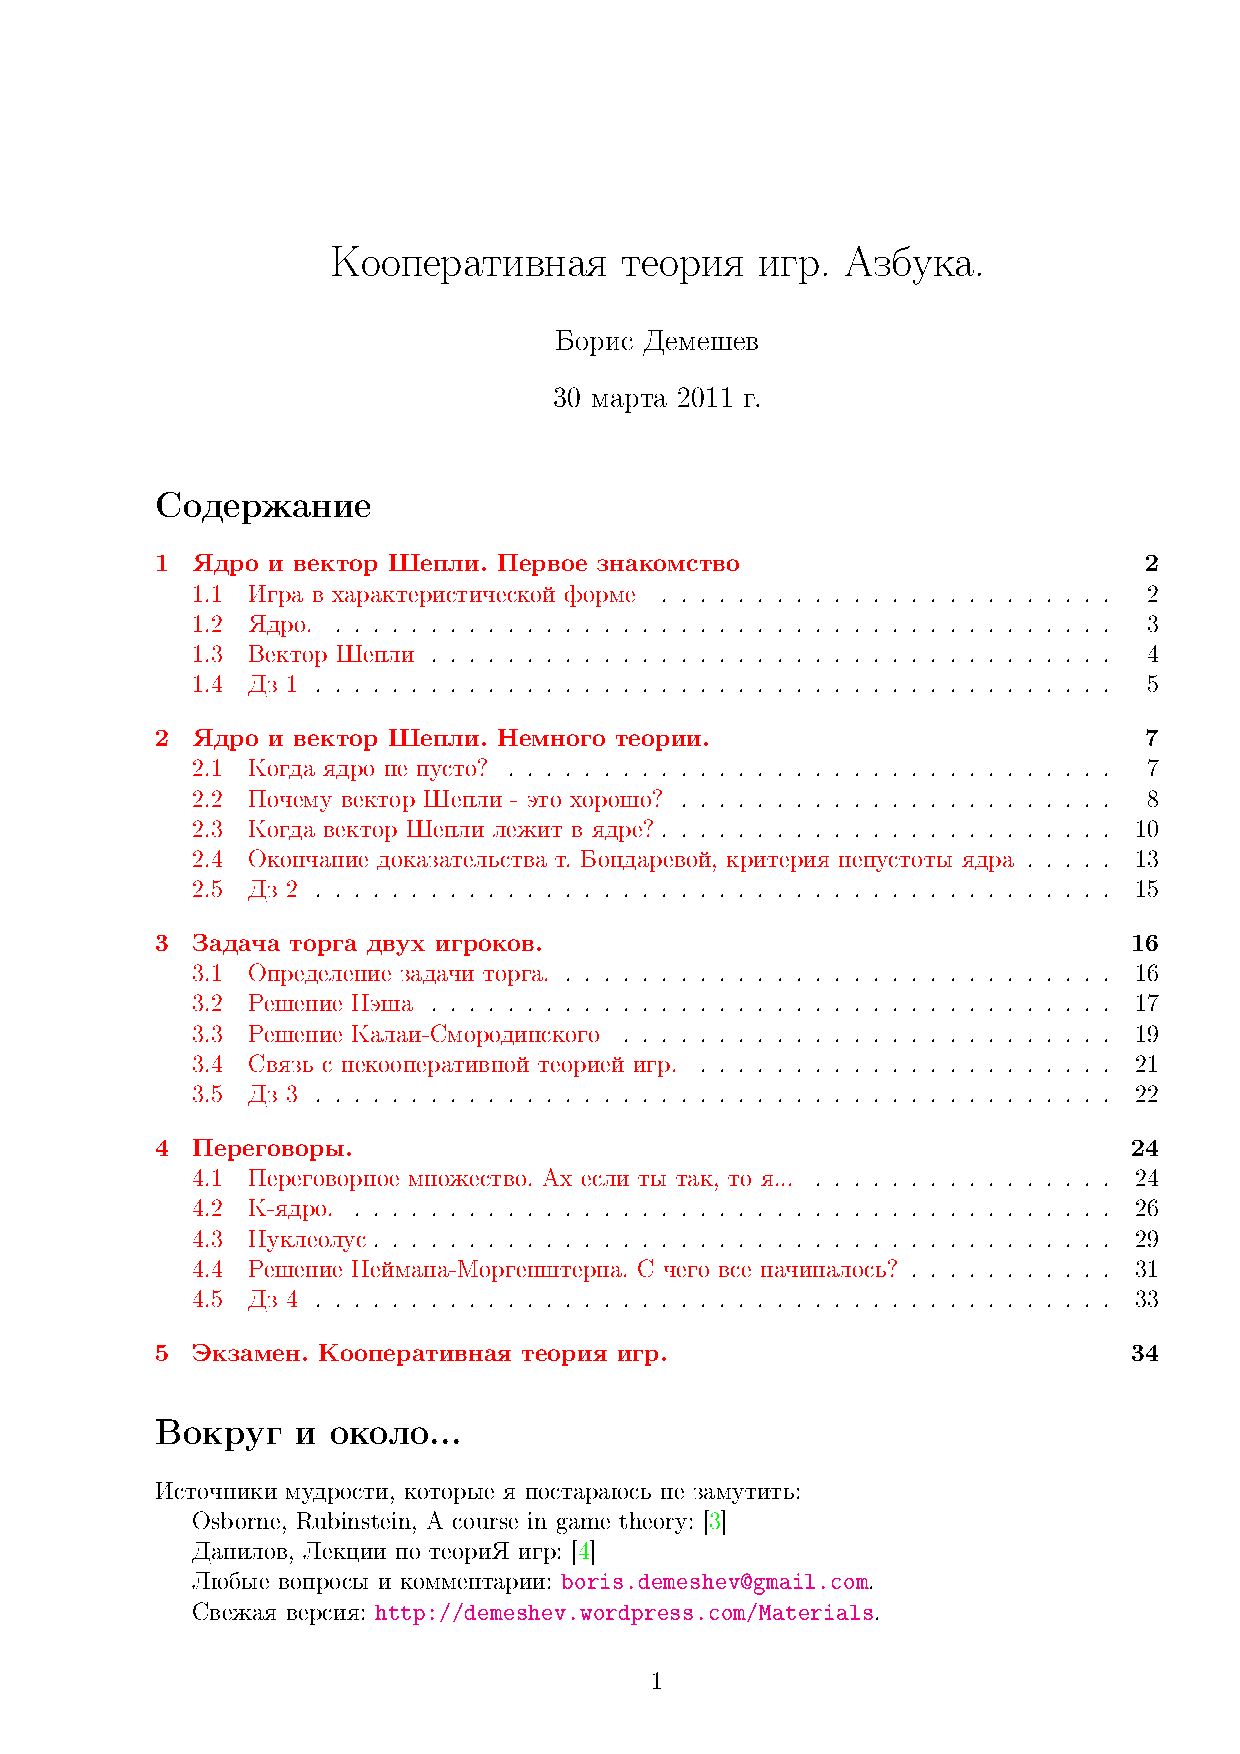
\includegraphics{coop_gt.2}
\end{figure}

Собственники труб и пропускная способность труб в таблице:

\begin{tabular}{|c|c|c|}

\hline 
Номер трубы & Пропускная способность & Владелец \\
\hline
1 & 2 л/час & Андрей \\
2 & 3 л/час & Борис \\
3 & 1 л/час & Володя \\
4 & 2 л/час & Борис \\
5 & 3 л/час & Андрей \\
\hline
\end{tabular}

Потребители нефти готовы платить 1 рубль за скорость передачи 1 литр/час. 

Найдите нуклеолус



\section{Экзамен. Кооперативная теория игр.}

Задача 1. ООН

Совет Безопасности ООН состоит из 15 членов. Пять членов Совета — постоянные (Россия, США, Великобритания, Франция и Китай), остальные десять членов - периодически меняются. Для принятия решения о применении санкций необходимо одобрение не менее 9 членов включая всех постоянных. В этой кооперативной игре выигрышем коалиции можно считать 1, если она может принять санкции, и 0, если не может.

Найдите вектор Шепли. Во сколько раз влияние постоянного члена сильнее, чем не постоянного?

Задача 2. Количество голосов

В стране N есть 5 провинций, разных по численности населения: 100, 100, 200, 300, 400 (тыс. чел.) Руководство страны состоит из 5 человек. Им даны голоса пропорционально численности провинции, т.е. 1, 1, 2, 3, 4 голоса, соответственно. Решение принимается, если за него подано не менее 8 голосов (из 11 возможных). В этой кооперативной игре выигрышем коалиции можно считать 1, если она может одобрить решение и 0, если не может.

а) Найдите вектор Шепли. Соответствует ли он численности населения?

б) (возможно явное использование компьютера). Подберите численности голосов так, чтобы вектор Шепли был максимально пропорционален численности населения.



Задача 3. Игра <<Мусор>>

Есть $n$ дворов. На каждом дворе скопился один мешок мусора. Вывоз одного мешка мусора стоит 1 рубль. Но можно же втихаря подкинуть его соседу! Поэтому: $v(N)=-n$ (т.к. большой коалиции придется по-любому убирать со своей территории $n$ мешков). Если какая-то коалиция захочет отсоединится от большой коалиции, то мы будем считать, что остаток большой коалиции будет играть против <<отколовшихся>>. Поэтому при $S\neq N$: $v(S)=|S|-n$, где $|S|$ - это численность коалиции $S$ (ровно столько мешков коалиции $S$ удастся выкинуть на соседские дворы).

Найдите ядро этой игры при произвольном $n$


Задача 4. Банковский вклад.

У Ани - 70 рублей, у Бори - 80 рублей, у Вовы - 150 рублей. Процентная ставка по вкладу: 5\% при сумме вклада в диапазоне $[0;100)$, 6\% при сумме вклада в диапазоне $[100;200)$ и 7\% при сумме вклада в диапазоне $[200;\infty)$. Если они соберутся вместе, то смогут расчитывать на ставку в 7\%. Как им поделить прибыль?

Найдите вектор шепли, нуклеолус, около-ядро (при поиске около-ядра придется уходить в отрицательные $\varepsilon$)


Задача 5. Добровольное страхование

Есть группа А из 100 человек. У каждого из них страховой случай (потеря 1-го рубля) наступает независимо с вероятностью 0.1. Они решили объединится и застраховать сами себя, так чтобы вероятность банкротства группы была равна всего 0.001. 
Есть группа Б из 100 человек. У каждого из них страховой случай (потеря 1-го рубля) наступает независимо с вероятностью 0.15. Они решили объединится и застраховать сами себя, так чтобы вероятность банкротства группы была равна всего 0.001. 

а) Каков должен быть резерв страховой компании А?

б)  Каков должен быть резерв страховой компании Б?

в) Две группы решили объединится и застраховать сами себя, так чтобы вероятность банкротства группы была равна всего 0.001. Каков должен быть резерв объединенной страховой компании? 

г) Как правильно поделить расходы между игроками в случае объедения двух страховых групп? (Найдите ядро, вектор Шепли, нуклеолус, К-ядро)

Задача 6. Обмен рисками.

Есть два фонда, А и Б. Активы А можно считать случайной величиной со средним 6 и дисперсией 5, активы Б - случайной величиной со средним 10 и дисперсией 15. Предположим для простоты, что они не коррелированы. Компании хотят обменятся активами так, чтобы средние не поменялись, а дисперсии упали. т.е. компания А отдает часть своих активов компании Б, а компания Б отдает часть своих активов компании А, возможно также, что одна из компаний платит другой какую-то сумму денег (безрисковый актив).

а) Нарисуйте на плоскости возможные комбинации дисперсий

б) Найдите решение Нэша и решение Калаи-Смородинского


Задача 7. Кое-какие свойства ядра

Рассмотрии игру 4-х игроков, $v$:

Ценность большой коалиции равна 2, $v(N)=2$

Ценность любой коалиции из 3-х игроков равна 1, $v(S)=1$ при $|S|=3$.

Ценность каждого отдельного игрока равна нулю, $v(i)=0$ при любых $i$.

$v(\{1,2\})=v(\{3,4\})=0$, ценность других коалиций из 2-х игроков равна 1.

а) Найдите ядро

б) Что произойдет с ядром, если ценность коалиции $\{1,3,4\}$ возрастет с 1 до 2?

в) Прокомментируйте то, что происходит с выигрышами 1-го, 3-го и 4-го игроков


Задача 8. Вектор Шепли и нуклеолус. Почувствуйте разницу!

Рассмотрим вариант игры <<Ботинки>>. В игре 4 игрока. У первого - 2 правых ботинка, у второго - 1 правый, у остальных - по одному левому. Полная пара стоит 1 рубль, отдельный ботинок ничего не стоит.

а) Найдите вектор Шепли и нуклеолус

б) Прокомментируйте разницу с игрой, в которой у первого игрока 1 правый ботинок.








%\input{coop_sol}

\printindex % печать предметного указателя здесь


\bibliography{/home/boris/Dropbox/tex_general/opit}
%\bibliography{e:/Documents/Dropbox/tex_general/opit}




\end{document}